\chapter{Signal Extraction}\label{ch:sig}
The number of observed signal events for the \Wpm and \Z bosons are determined by a simultaneous fit of \Wp, \Wm, and \Z. This fit utilizes distributions of \mt for \Wpm and \mll for \Z, using simulated distributions for most of the signal and background processes, to extract a production rate for each of the processes. Transverse mass, \mt, is described in Equation~\ref{eq:mt}.
\begin{equation}
\mt = \sqrt{ 2 \pt^{\ell} \met ( 1 - \cos[\Delta\phi( {\vec \ell},\met ) ] ) }
\label{eq:mt}
\end{equation}
The \mll distribution for the \zll signal processes are taken from simulation, with the appropriate lepton momentum scale and efficiency scale factors applied. The \mt distributions for the \wlnu signals additionally require the application of hadronic recoil corrections.

Uncertainties on normalization are included as nuisance parameters, and uncertainties on kinematic observables such as lepton \pt are propagated through the \mt or \mll distribution as shape uncertainties. Details of the signal and background \mt and \mll distribution modeling are provided in this chapter, as well as the results of the signal extraction fits.

%%%%%%%%%%%%%%%%%%%%%%%%%%%%%%%%%%%%%%%%%%%%
%%%               background
%%%%%%%%%%%%%%%%%%%%%%%%%%%%%%%%%%%%%%%%%%%%
\section{Background Modeling}\label{ch:sig:bkg}
Backgrounds are estimated from both simulation and data-driven sources. Simulated backgrounds include the \ttbar and various electroweak processes, and include the appropriate normalization factors for prefiring and efficiency. Backgrounds to \W and \Z can include \ttbar and diboson (\W\W, \W\Z, \Z\Z) processes contributing one or two isolated leptons, respectively. The DY background to the \W is from a \zmm or \zee decay with only one lepton being in the detector volume, or the \ztt with one of the $\tau$ decaying leptonically. \ztt with leptonic $\tau$ decays is also a background to the \Z. The \wtaunu, with leptonic $\tau$ decay also contributes to the \W backgrounds.

 
\subsubsection{QCD Background}\label{ch:w:qcd}
The largest background of the \wlnu lepton + \met signature is from QCD multijet background. The primary contributions are heavy-flavor decays and $\gamma$+jets with photon conversion to electrons. 
There are no simulations of the QCD background available for the datasets used in this analysis, therefore a data-driven method of estimating the \mt distribution from QCD sources is used. A QCD-enriched region composed of non-isolated leptons is obtained from data by inverting the lepton isolation criteria in the lepton ID cuts and subtracting the expected \mt distributions described by simulation due to \W signal and other background processes. The QCD multijet background \mt distribution is taken from the $0.30 < \mathrm{Iso} < 0.45$ control region. The region $0.15 < \mathrm{Iso} < 0.30$ is excluded due to high levels of \W signal contamination (approx 30\% \W). The \mt distributions are generally stable over different isolation ranges.


\section{Uncertainties}\label{ch:unc}
Uncertainties on corrections are propaged to the final obserable distributions \mt and \mll. These include variations on the lepton momentum scale factors, recoil corrections, prefiring probability, and lepton efficiency.
An uncertainty on the QCD multijet shape due to the choice of control region is estimated by using an second isolation range and taking the difference as the shape uncertainty. The main QCD \mt shape is from the $0.30 < \mathrm{Iso} < 0.45$ region, and the shape uncertainty is derived from the difference with respect to the \mt distribution in $0.45 < \mathrm{Iso} < 0.60$.

\section{Summary}

The observed yields resulting from the signal extraction fits for all signal and background processes are listed in Table~\ref{tab:yield:ele:5} (Table~\ref{tab:yield:ele:13}) for the electron channels and Table~\ref{tab:yield:mu:5} (Table~\ref{tab:yield:mu:13}) for the muon channels at \serag (\serah). Quoted uncertainties include both statistical and systematic sources.

Figures showing the \Zmm and \Zee \mll distributions are shown in Figure~\ref{fig:z:z:5} for \serag and Figure~\ref{fig:z:z:13} for \serah. Distributions of \mt for \W fits are shown in Figure~\ref{fig:signal_wp} for \Wp and Figure~\ref{fig:signal_wm} for \Wm.

 
\begin{table}[htbp]
\centering
\newcolumntype{x}{D{,}{\,\pm\,}{3.3}}
\begin{tabular}{l@{\hspace*{1.5cm}}x{c}@{\hspace*{1.5cm}}x{c}@{\hspace*{1.5cm}}x}
Process   	      &   \multicolumn{1}{c}{\zee} &&  \multicolumn{1}{c}{\wep} &&  \multicolumn{1}{c}{\wem}  	    \\
%\cline{2-2}\cline{4-4}
\hline
Data                &   \multicolumn{1}{c}{$47734$}   && \multicolumn{1}{c}{$438547$}    && \multicolumn{1}{c}{$289179$}    \\
\hline
\hline
Signal                &   747323 , 862  &&    398952,  338    &&  252850 ,  274  \\    
QCD multijet          &   0 , 0   &&   27181 ,  333  &&  25968 ,  305  \\  
\ttbar             &   32 ,  3  &&    679 ,  11  &&  677 ,  11  \\    
Drell--Yan  	      &   508 ,  9  &&    11734 ,  176   &&  9684 ,  173  \\     
$\W \rightarrow \tau\nu$     &   < 1 &&    7372 ,  165    &&  5649 ,  159  \\    
Diboson               &   54 ,  5  &&    88 ,  1    &&  80 ,  1  \\    
\end{tabular}
\caption{Best-fit yields from various processes in \Z, \Wp, and \Wm boson with electron final states at \sg. Uncertainties shown are a combination of systematic and statistical.}
\label{tab:yield:ele:5}
\end{table}



\begin{table}[htbp]
\centering
\newcolumntype{x}{D{,}{\,\pm\,}{3.3}}
\begin{tabular}{l@{\hspace*{1.5cm}}x{c}@{\hspace*{1.5cm}}x{c}@{\hspace*{1.5cm}}x}
Process   	      &   \multicolumn{1}{c}{\zmm} &&  \multicolumn{1}{c}{\wmp} &&  \multicolumn{1}{c}{\wmm}  	    \\
%\cline{2-2}\cline{4-4}
\hline
Data                &   \multicolumn{1}{c}{$79345$}   && \multicolumn{1}{c}{$672817$}    && \multicolumn{1}{c}{$428156$}    \\
\hline
\hline
Signal                &   79076 ,  249  &&    626189,  554    &&  389637 ,  420  \\    
QCD multijet          &   0 , 0   &&   12496 ,  238  &&  12616 ,  162  \\  
\ttbar             &   49 ,  5  &&    828 ,  13  &&  836 ,  14  \\    
Drell--Yan  	      &   126 ,  3  &&    33295 ,  258   &&  25066 ,  194  \\     
$\W \rightarrow \tau\nu$     &   < 1 &&    13268 ,  232    &&  8450 ,  159  \\    
Diboson               &   88 ,  9  &&    125 ,  2    &&  112 ,  2  \\    
\end{tabular}
\caption{Best-fit yields from various processes in \Z, \Wp, and \Wm bosons with muon final states at \sg. Uncertainties shown are a combination of systematic and statistical.}
\label{tab:yield:mu:5}
\end{table}

\begin{table}[htbp]
\centering
\newcolumntype{x}{D{,}{\,\pm\,}{3.3}}
\begin{tabular}{l@{\hspace*{1.5cm}}x{c}@{\hspace*{1.5cm}}x{c}@{\hspace*{1.5cm}}x}
Process   	      &   \multicolumn{1}{c}{\zee} &&  \multicolumn{1}{c}{\wep} &&  \multicolumn{1}{c}{\wem}  	    \\
%\cline{2-2}\cline{4-4}
\hline
Data                &   \multicolumn{1}{c}{$76229$}   && \multicolumn{1}{c}{$709630$}    && \multicolumn{1}{c}{$578135$}    \\
\hline
\hline
Signal                &   73800 ,  1320  &&    605443,  372    &&  477096 ,  342  \\    
QCD multijet          &   0 , 0    &&     77133 ,  475  &&  76496 ,  442  \\  
\ttbar             &   203 ,  21  &&    5833 ,  94  &&  5871 ,  94  \\    
Drell--Yan  	      &   748 ,  14  &&    21222 ,  167   &&  18653 ,  153  \\     
$\W \rightarrow \tau\nu$     &   < 1 &&    9434 ,  109    &&  7422 ,  93  \\    
Diboson               &   93 ,  9  &&    240 ,  3    &&  231 ,  3  \\    
\end{tabular}
\caption{Best-fit yields from various processes in \Z, \Wp, and \Wm bosons with electron final states at \sh. Uncertainties shown are a combination of systematic and statistical.[estimating QCD yield for Z with e-mu selection, will add to table]}
\label{tab:yield:ele:13}
\end{table}


\begin{table}[htbp]
\centering
\newcolumntype{x}{D{,}{\,\pm\,}{3.3}}
\begin{tabular}{l@{\hspace*{1.5cm}}x{c}@{\hspace*{1.5cm}}x{c}@{\hspace*{1.5cm}}x}
Process   	      &   \multicolumn{1}{c}{\zmm} &&  \multicolumn{1}{c}{\wmp} &&  \multicolumn{1}{c}{\wmm}  	    \\
%\cline{2-2}\cline{4-4}
\hline
Data                &   \multicolumn{1}{c}{$128713$}   && \multicolumn{1}{c}{$1014670$}    && \multicolumn{1}{c}{$795518$}    \\
\hline
\hline
Signal                &   126473 ,  2261  &&    902641,  666    &&  696182 ,  586  \\    
QCD multijet          &   0 , 0    &&   50374 , 337  &&  46450 ,  315  \\  
\ttbar             &   326 ,  34  &&    6558 ,  100  &&  6148 ,  89  \\    
Drell--Yan  	      &   204 ,  4  &&    55084 ,  305   &&  46742 ,  241  \\     
$\W \rightarrow \tau\nu$     &   < 1  &&    17802 ,  229    &&  14285 ,  170  \\    
Diboson               &   151 ,  15  &&    317 ,  4    &&  296 ,  4  \\    
\end{tabular}
\caption{Best-fit yields from various processes in \Z, \Wp, and \Wm bosons with muon final states at \sh. Uncertainties shown are a combination of systematic and statistical[estimating QCD yield for Z with e-mu selection, will add to table].}
\label{tab:yield:mu:13}
\end{table}

\begin{figure}
\centering
\begin{subfigure}{.50\textwidth}
\centering
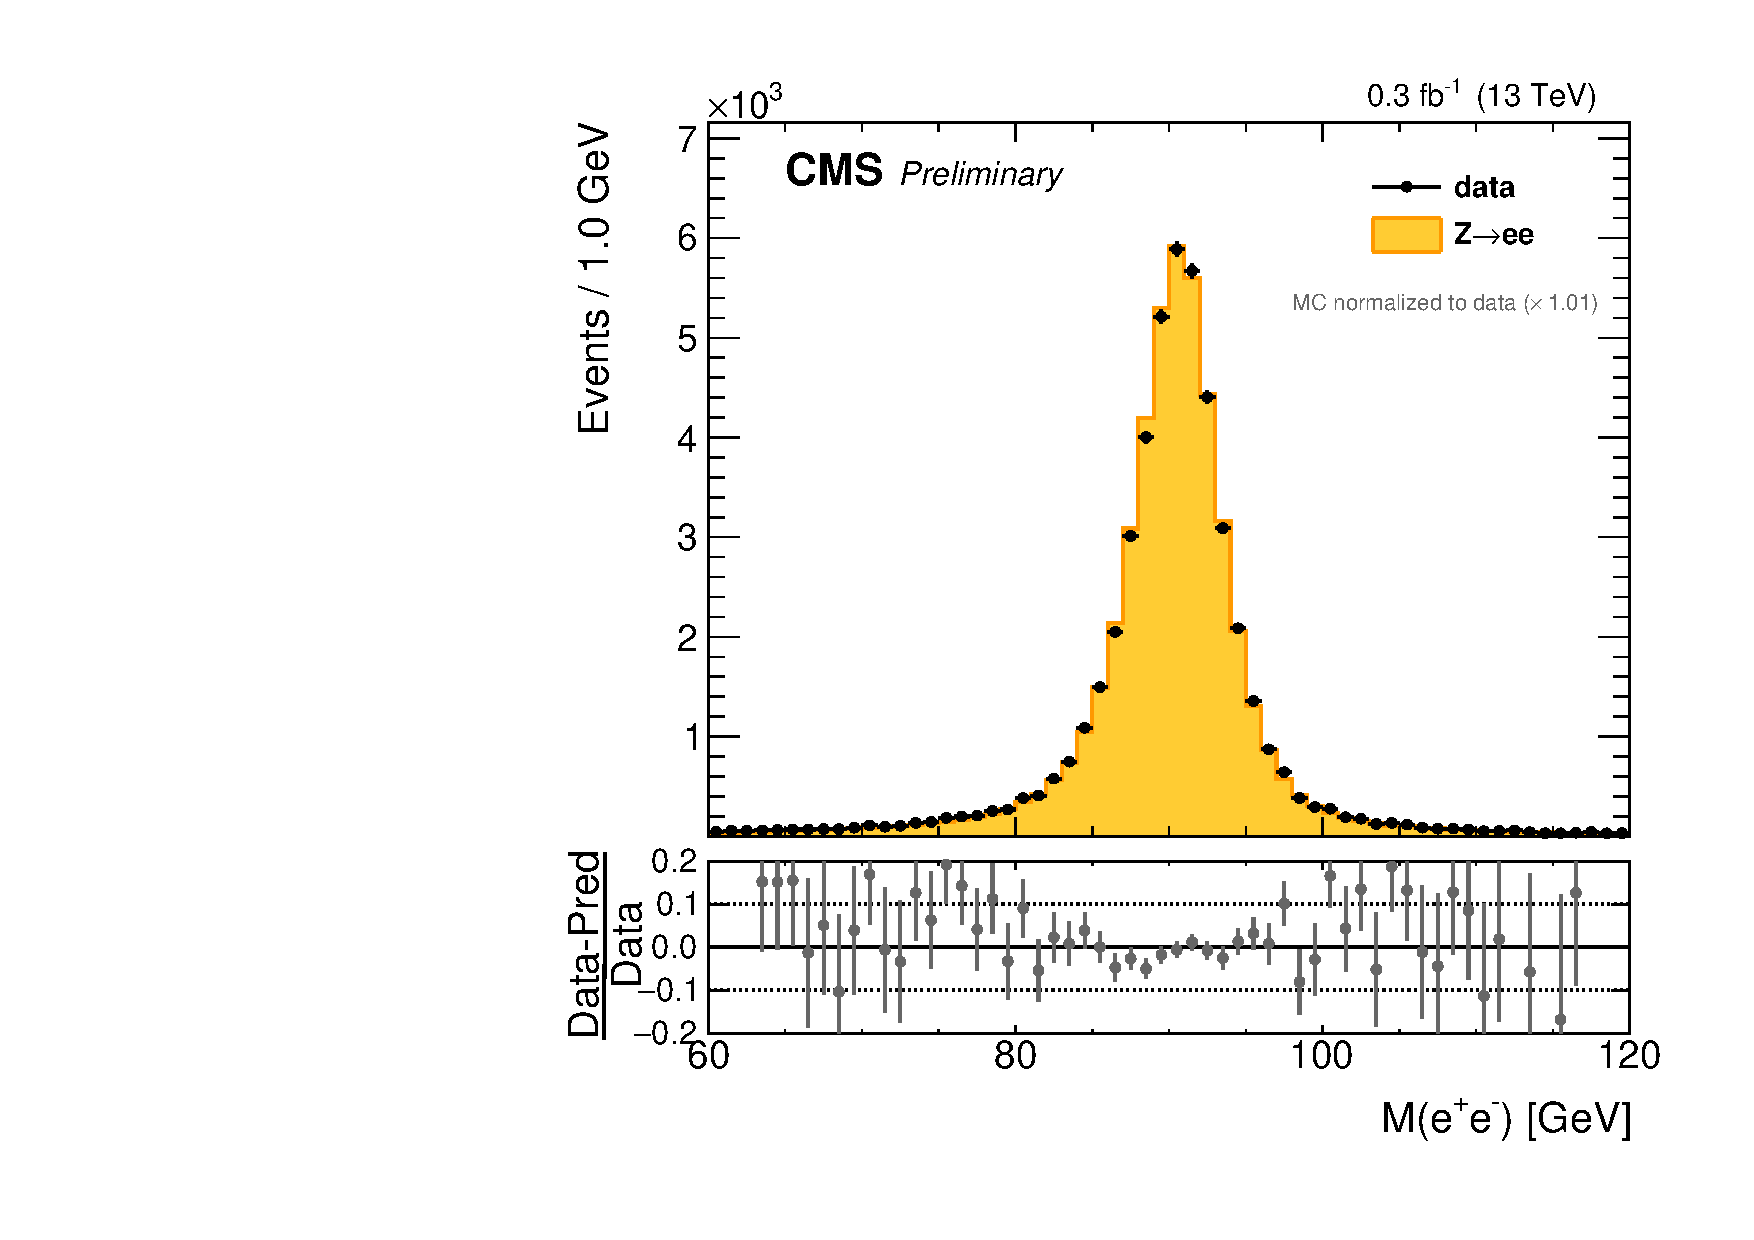
\includegraphics[width=\linewidth]{plots/Z/5tev/zee_norm.pdf}
\end{subfigure}%
\centering
\begin{subfigure}{.50\textwidth}
\centering
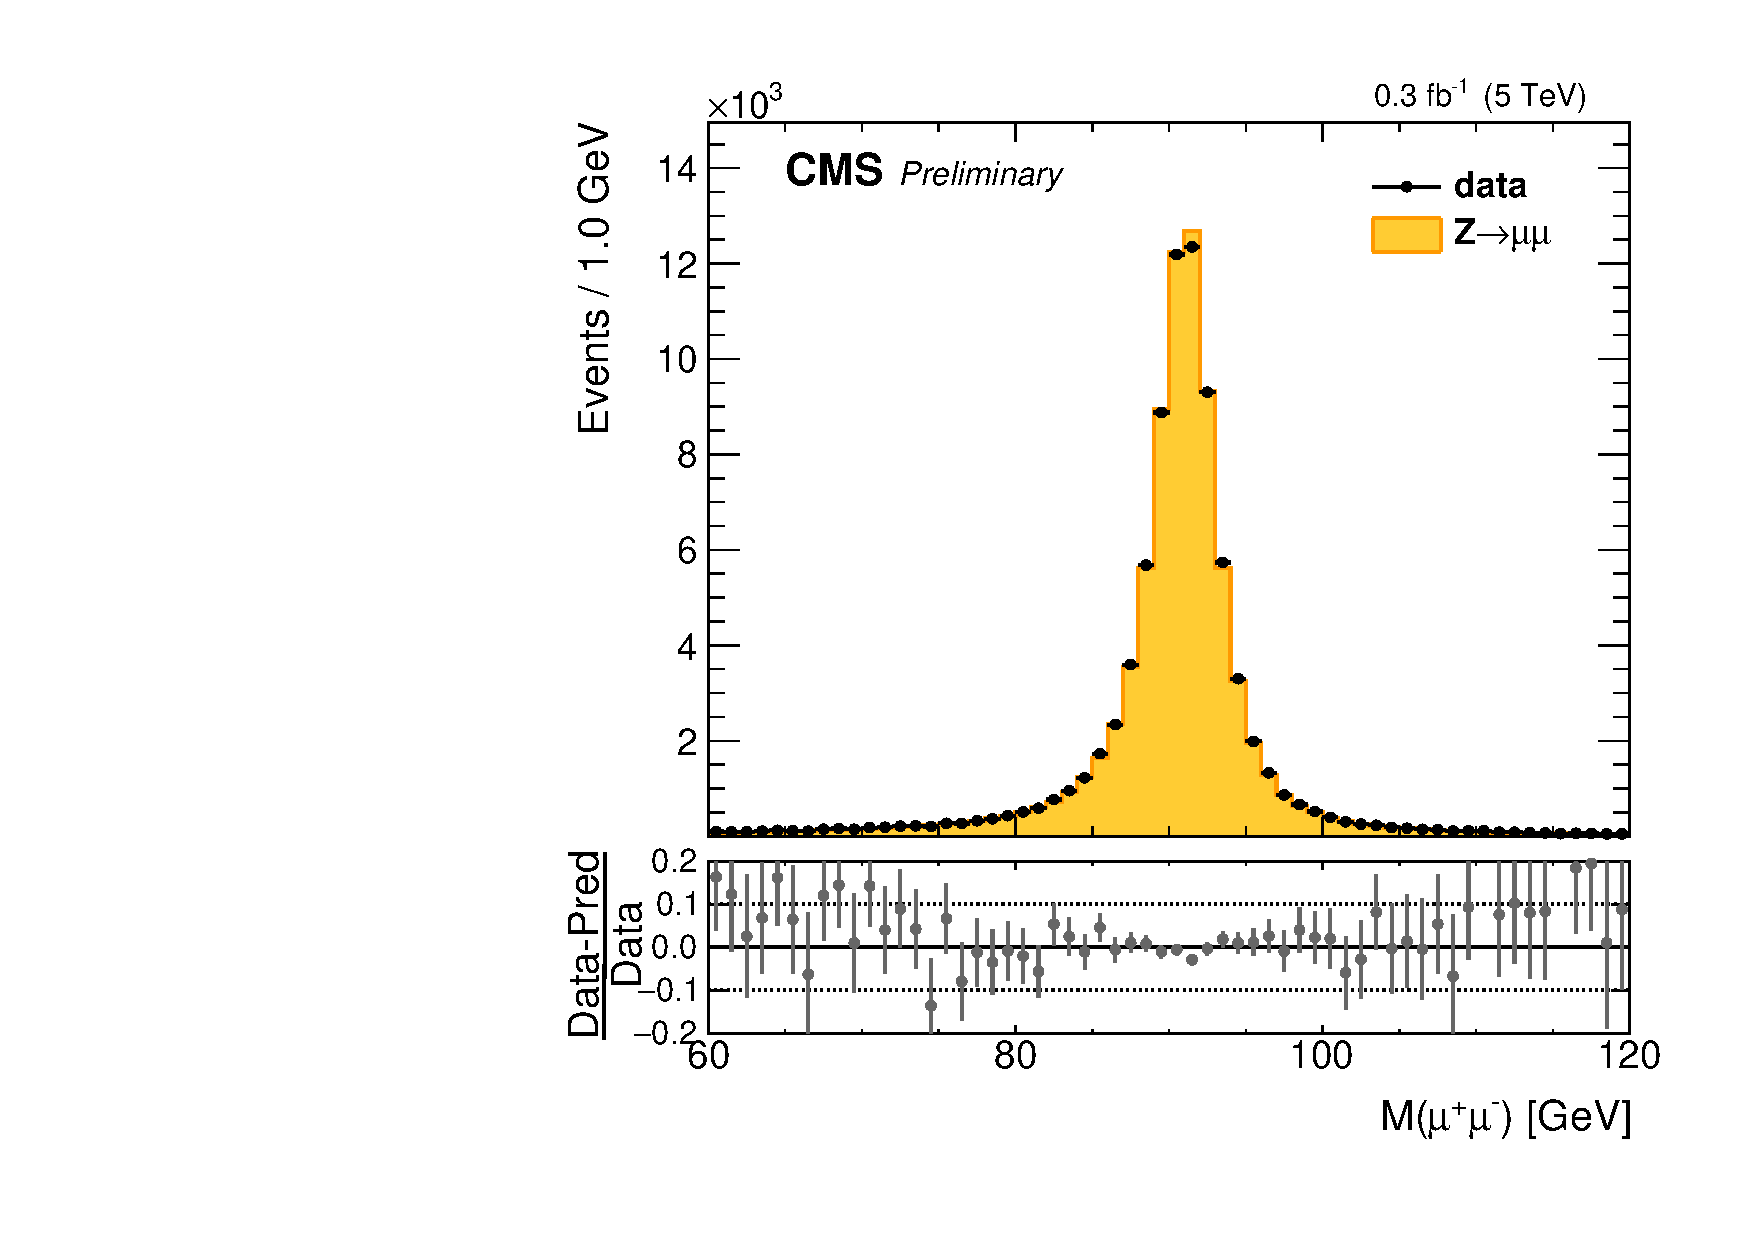
\includegraphics[width=\linewidth]{plots/Z/5tev/zmm.pdf}
\end{subfigure}%
\\
\centering
\begin{subfigure}{.50\textwidth}
\centering
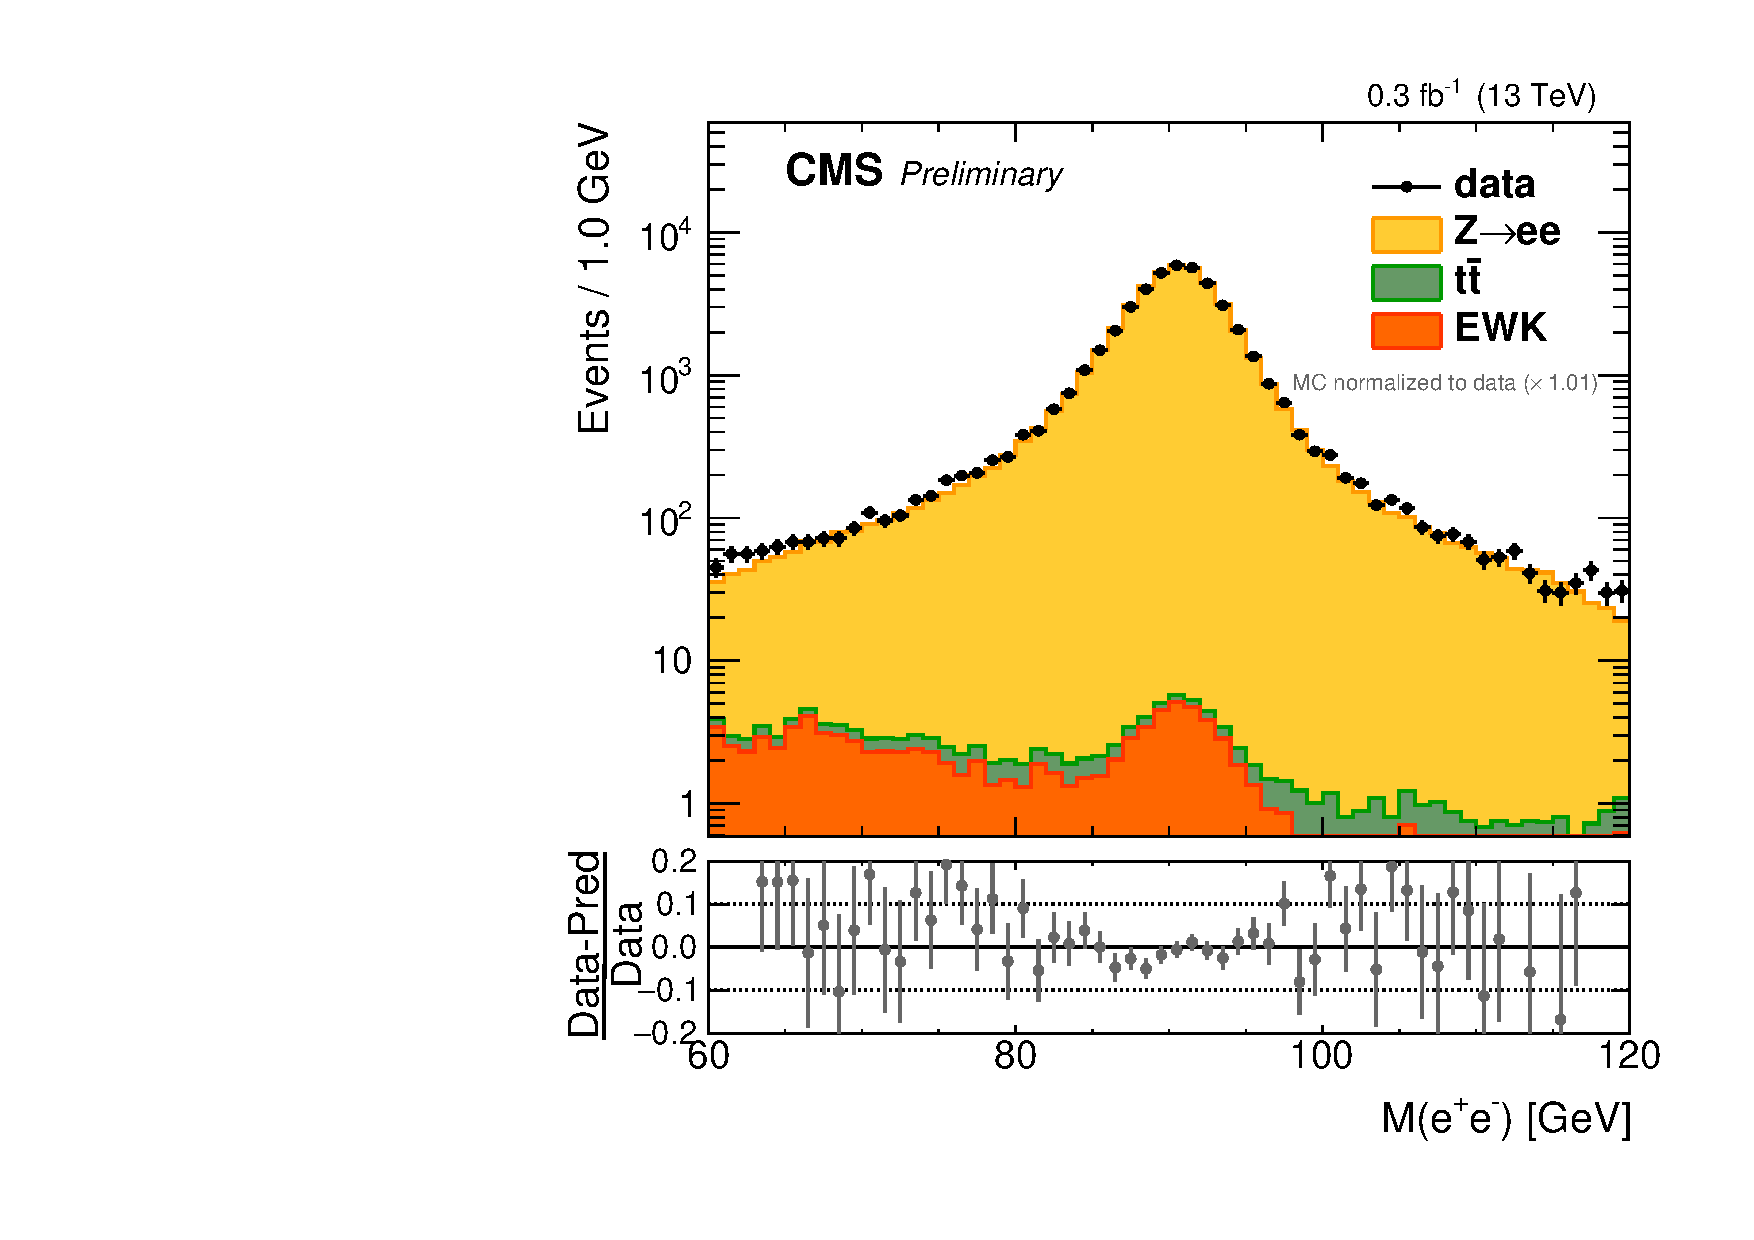
\includegraphics[width=\linewidth]{plots/Z/5tev/zeelog_norm.pdf}
\end{subfigure}%
\centering
\begin{subfigure}{.50\textwidth}
\centering
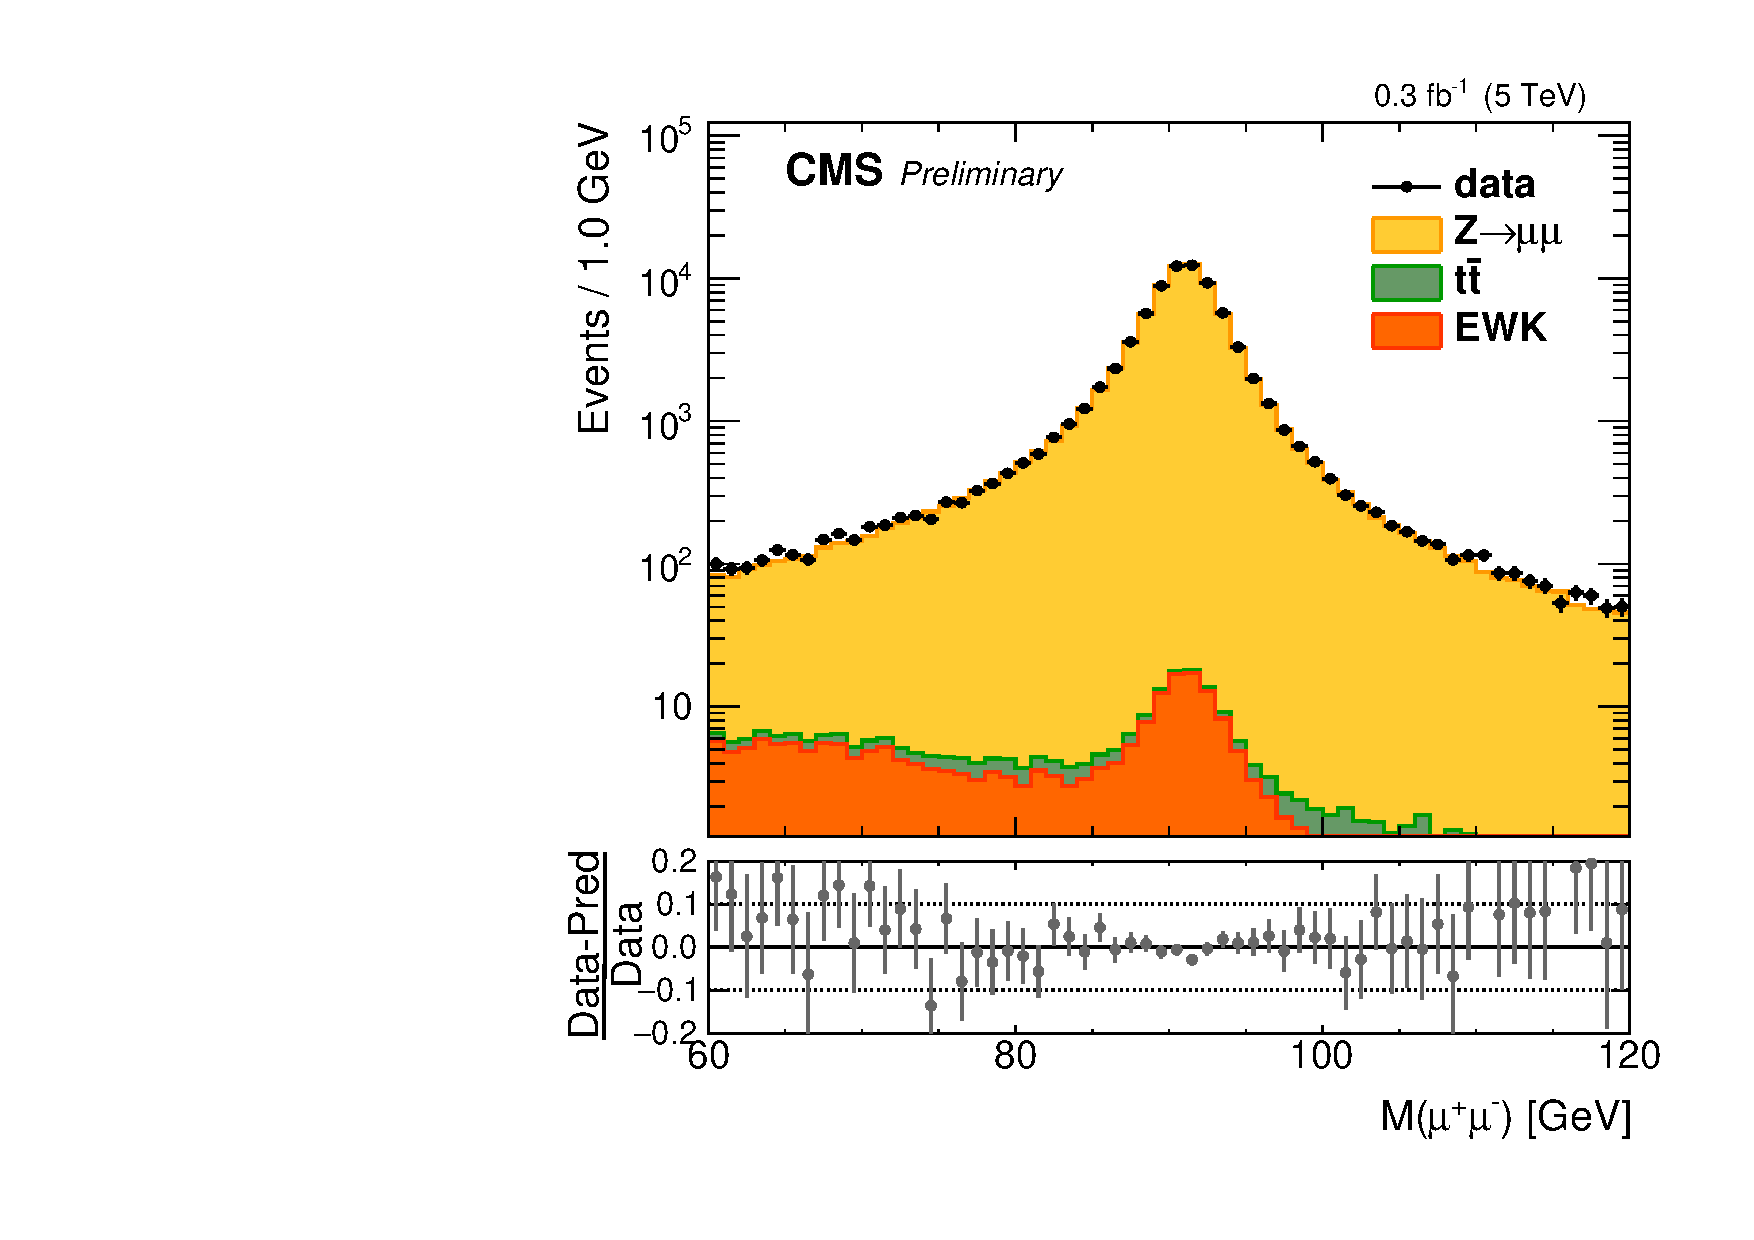
\includegraphics[width=\linewidth]{plots/Z/5tev/zmmlog.pdf}
\end{subfigure}%
\caption{The \mll distributions for \zee (left) and \zmm (right) at \sg. The simulated events have been normalized to data.}
\label{fig:z:z:5}
\end{figure}

\begin{figure}
\centering
\begin{subfigure}{.50\textwidth}
\centering
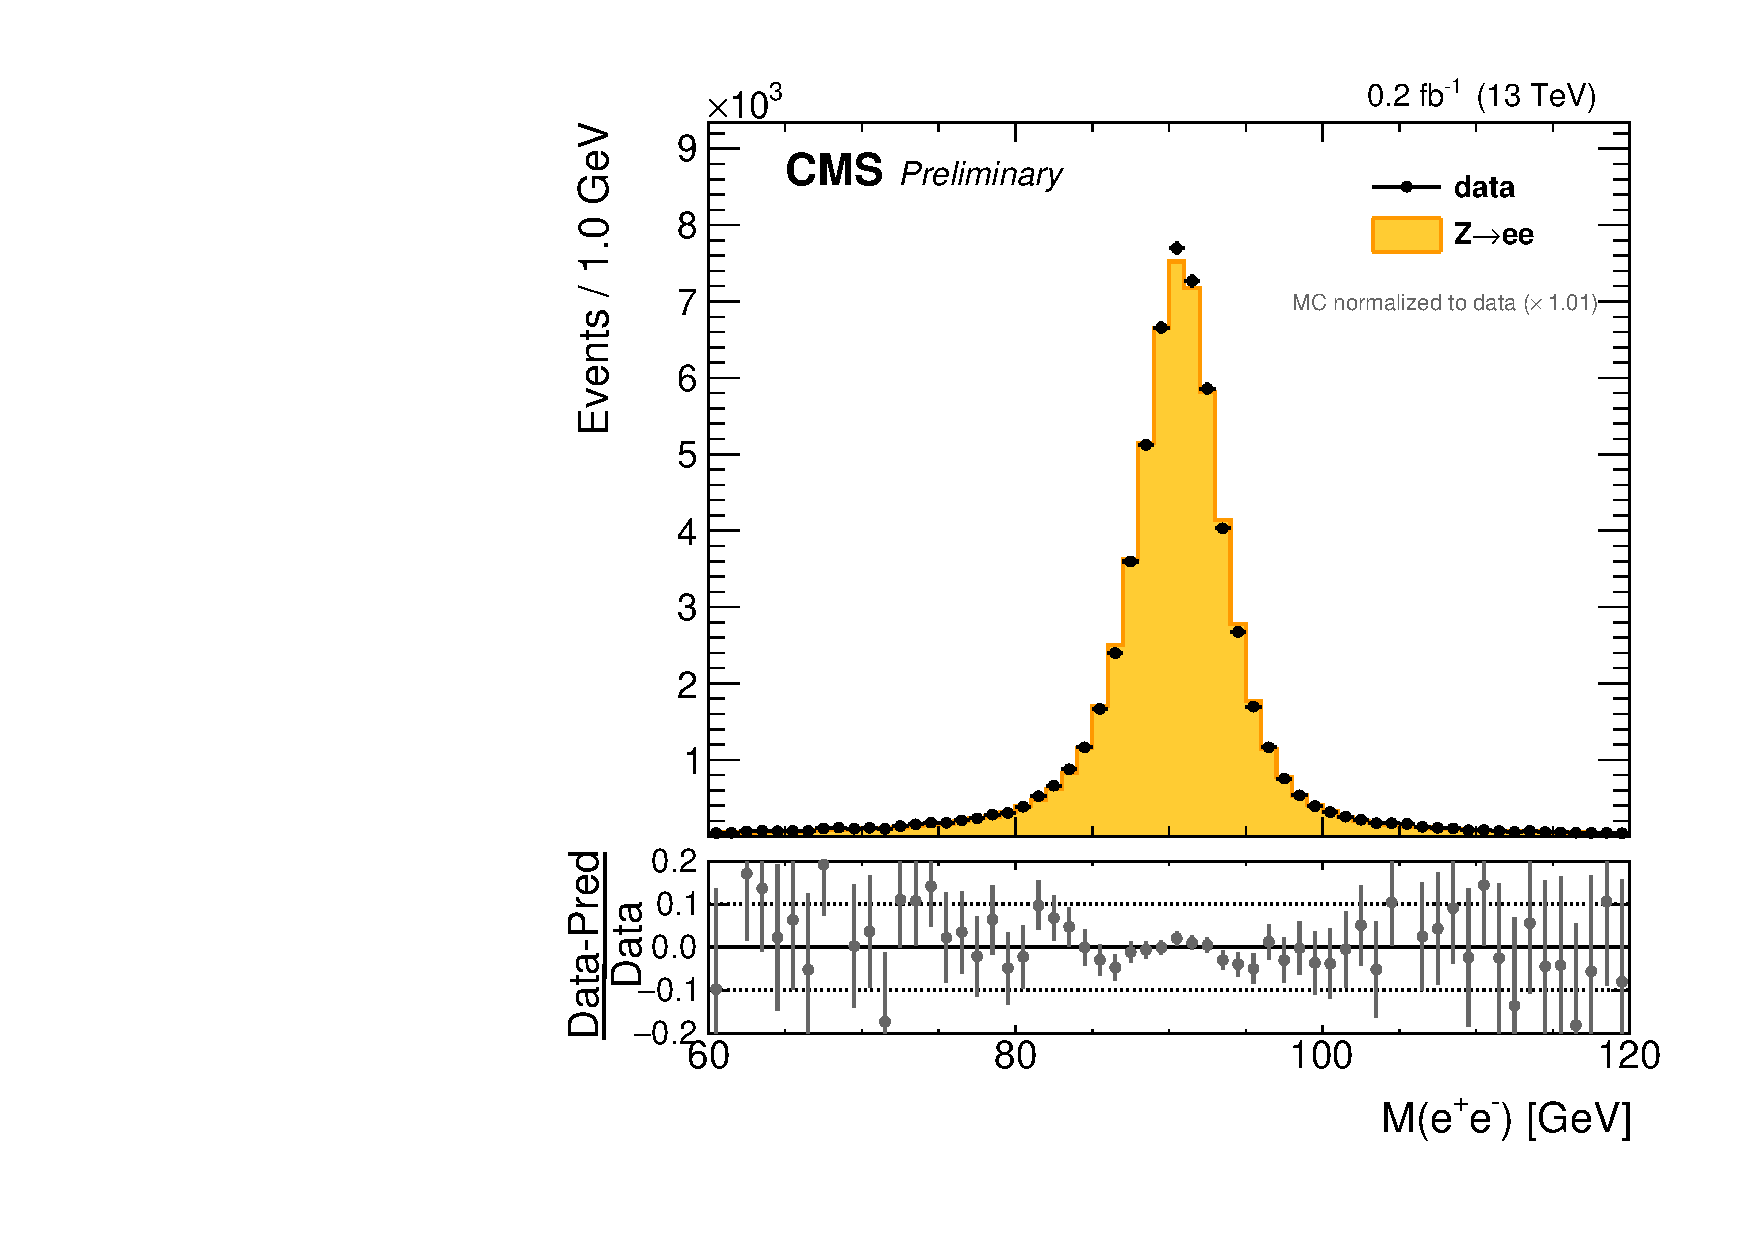
\includegraphics[width=\linewidth]{plots/Z/13tev/zee_norm.pdf}
\end{subfigure}%
\centering
\begin{subfigure}{.50\textwidth}
\centering
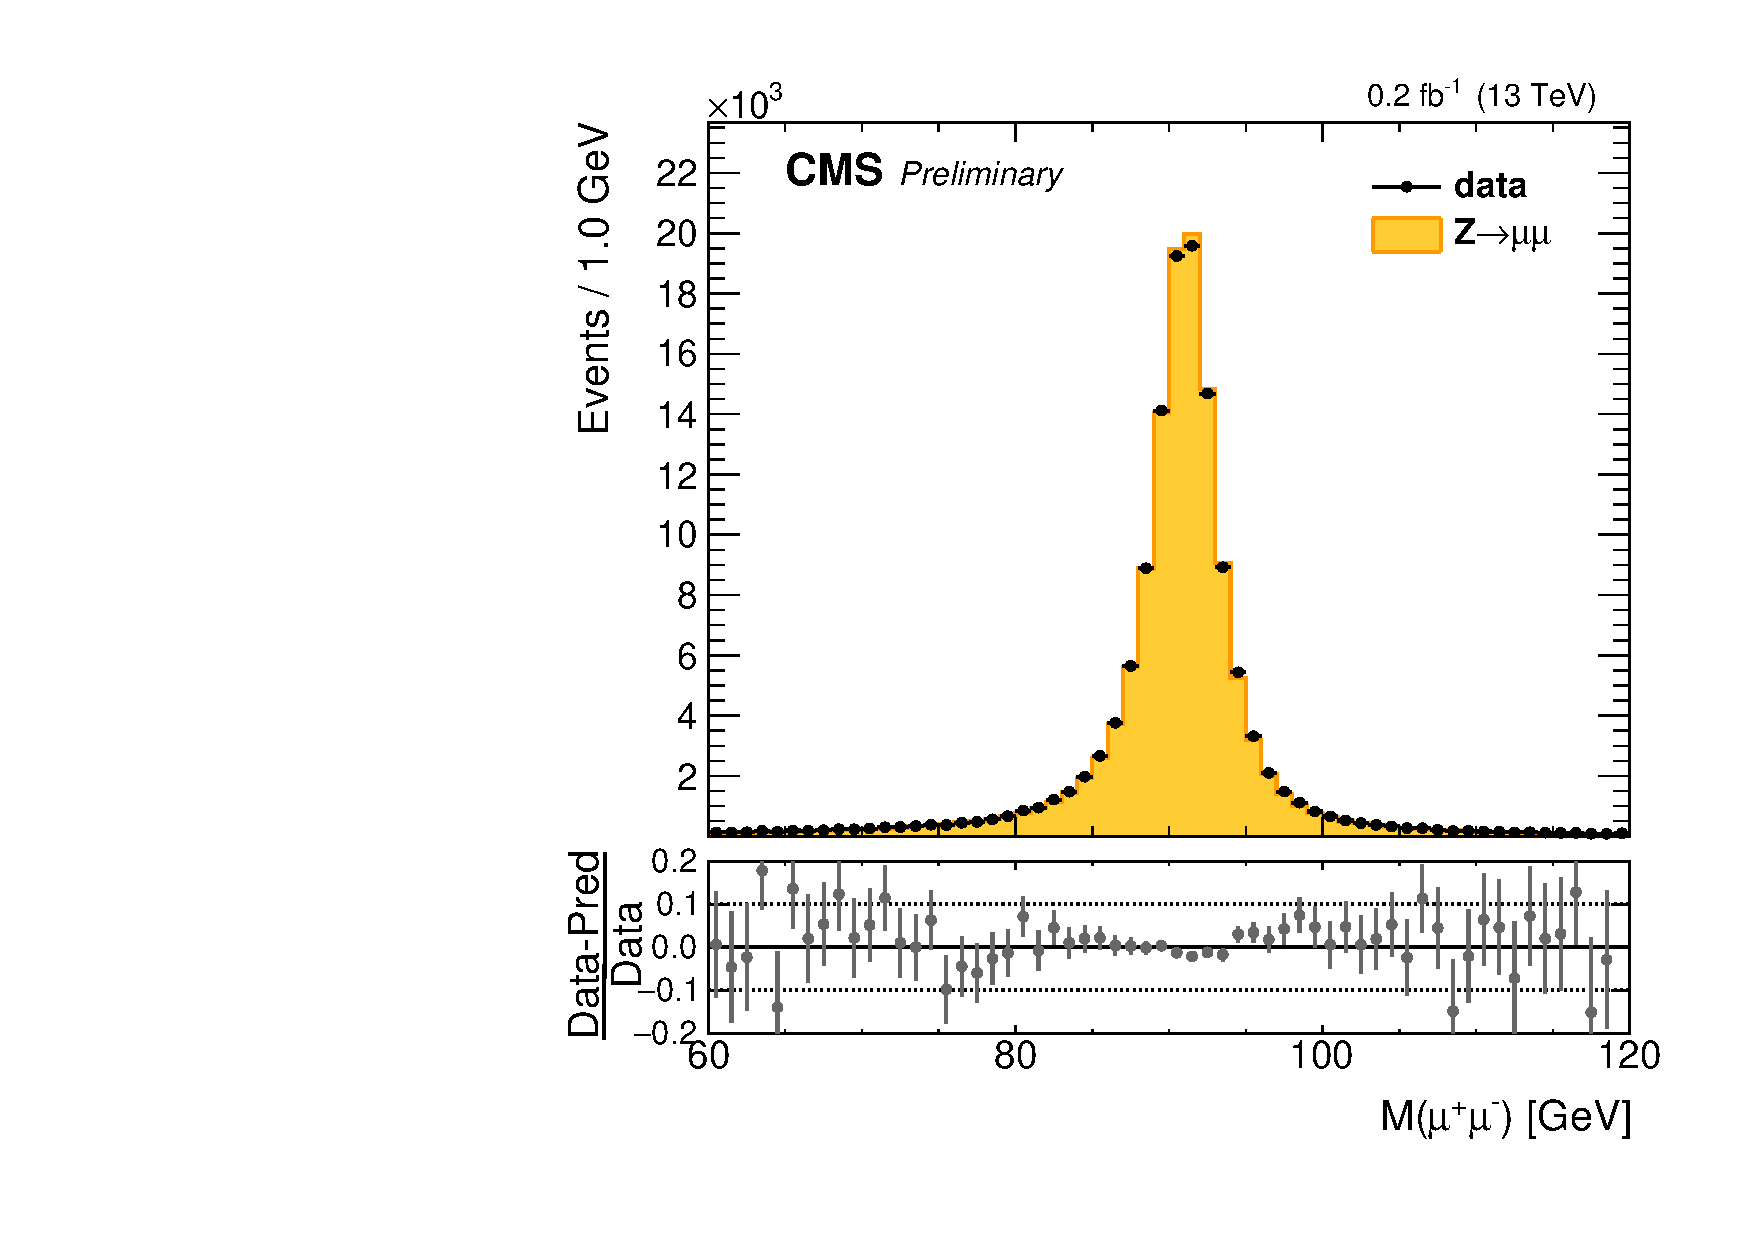
\includegraphics[width=\linewidth]{plots/Z/13tev/zmm.pdf}
\end{subfigure}%
\\
\centering
\begin{subfigure}{.50\textwidth}
\centering
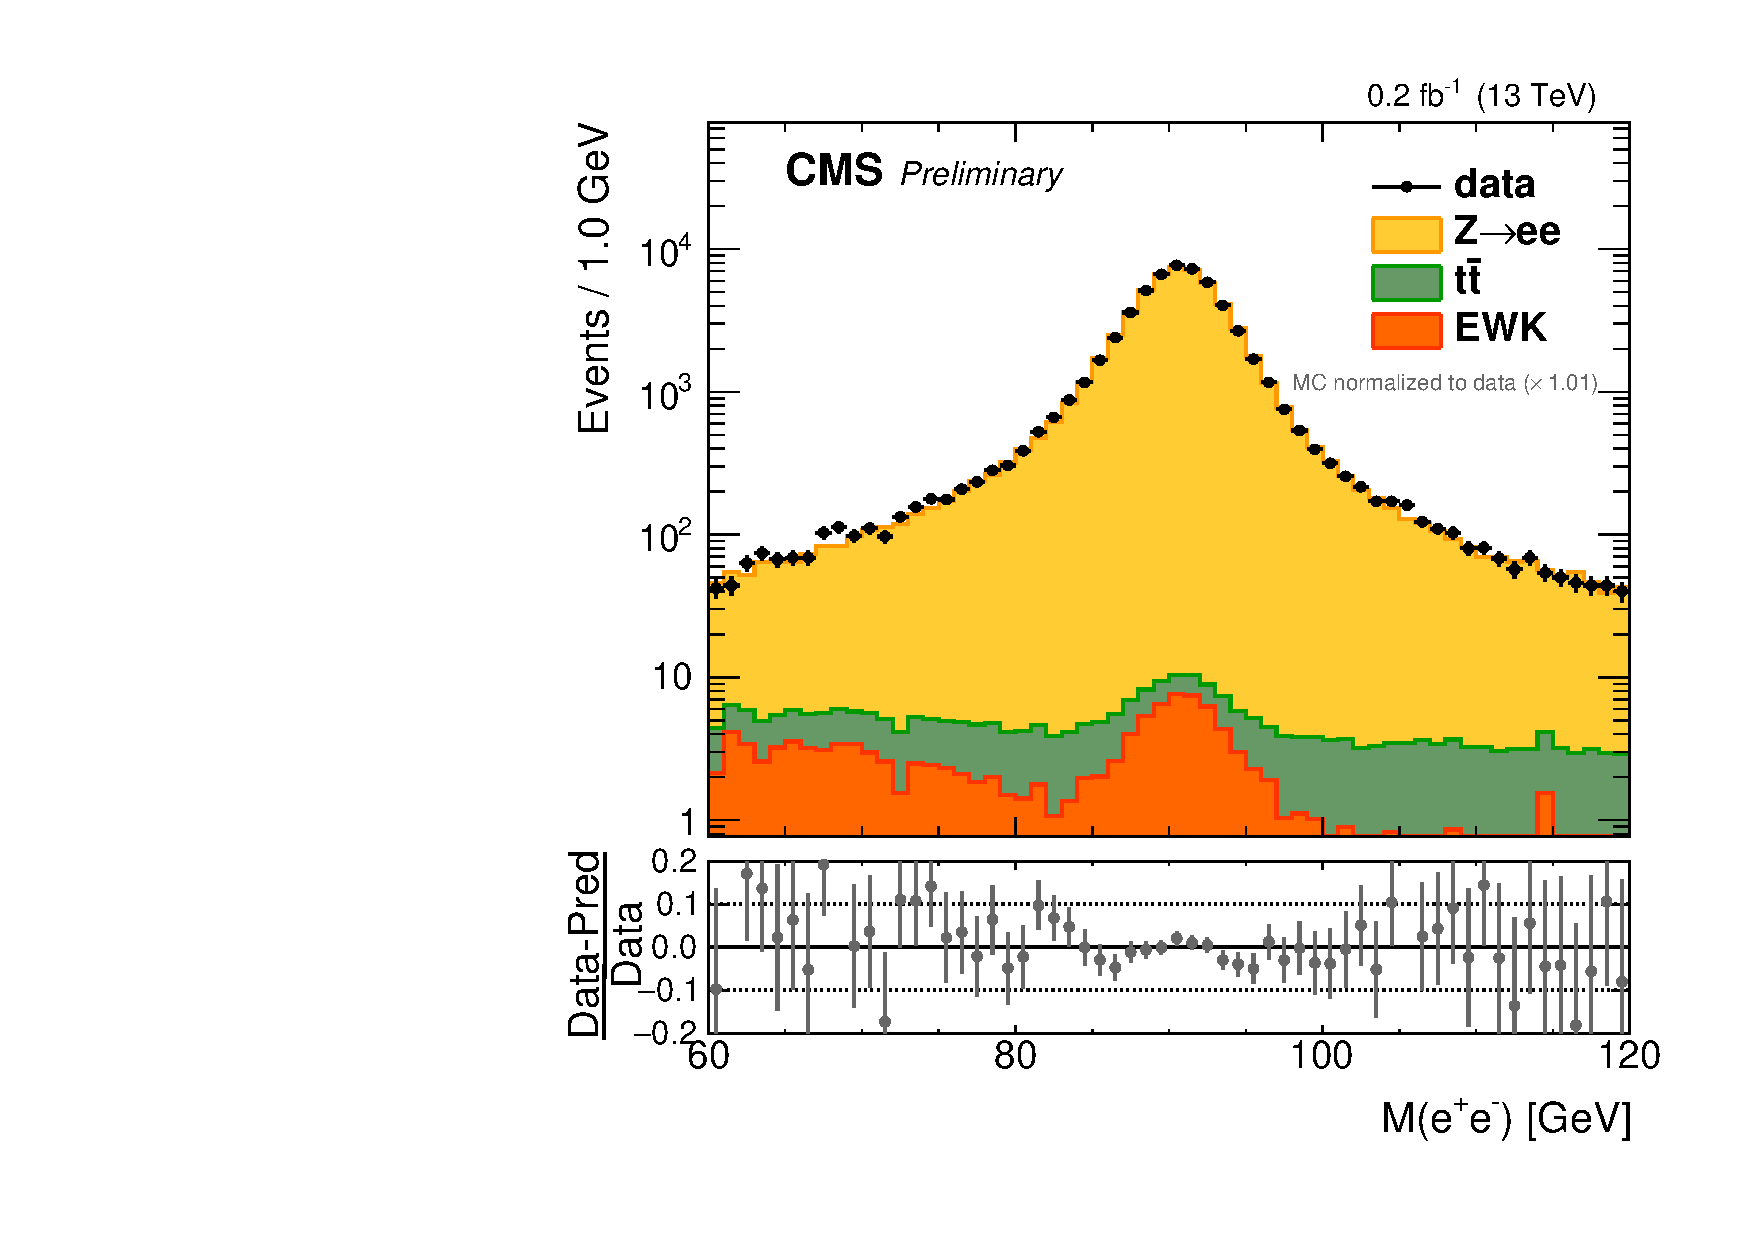
\includegraphics[width=\linewidth]{plots/Z/13tev/zeelog_norm.pdf}
\end{subfigure}%
\centering
\begin{subfigure}{.50\textwidth}
\centering
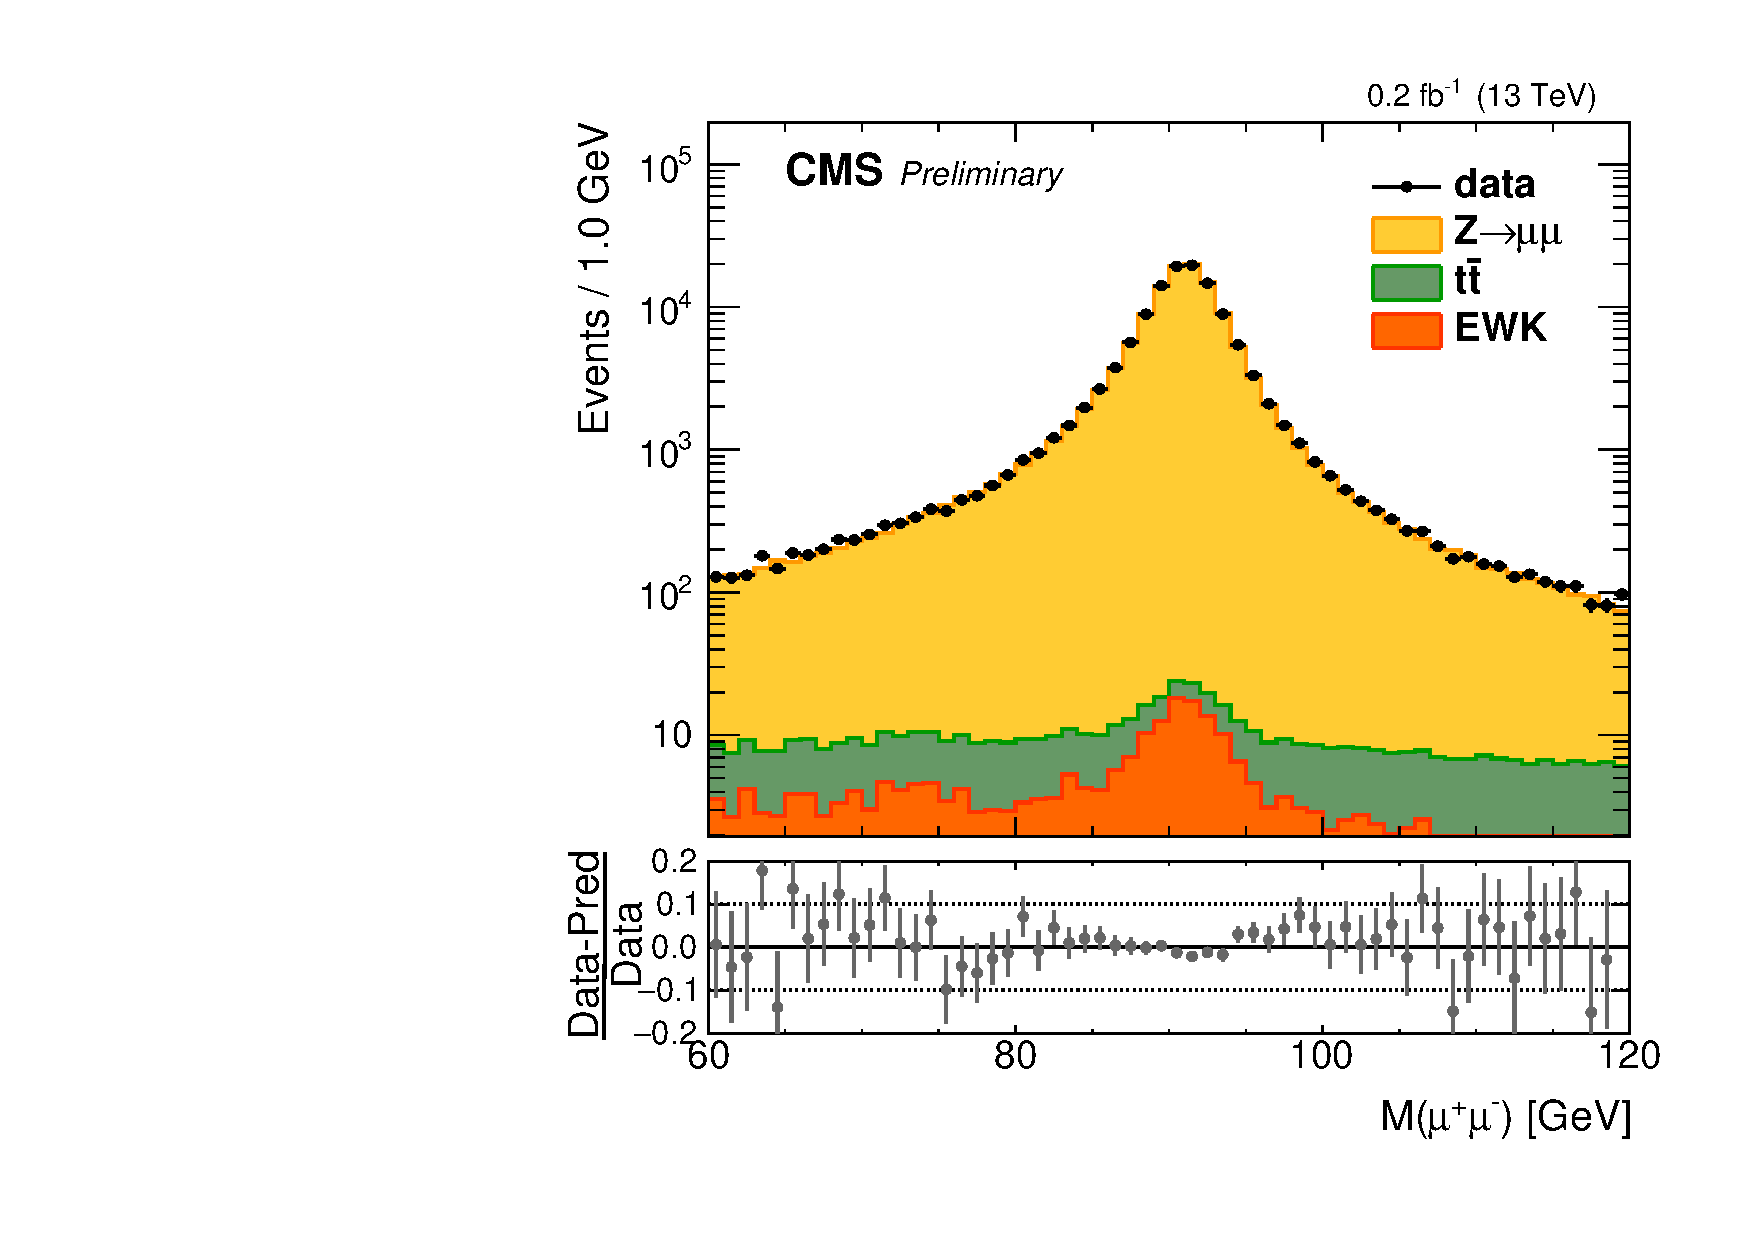
\includegraphics[width=\linewidth]{plots/Z/13tev/zmmlog.pdf}
\end{subfigure}%
\caption{The \mll distributions for \zee (left) and \zmm (right) at \sh. The simulated events have been normalized to data.}
\label{fig:z:z:13}
\end{figure}

\begin{figure*}[htb]
\centering
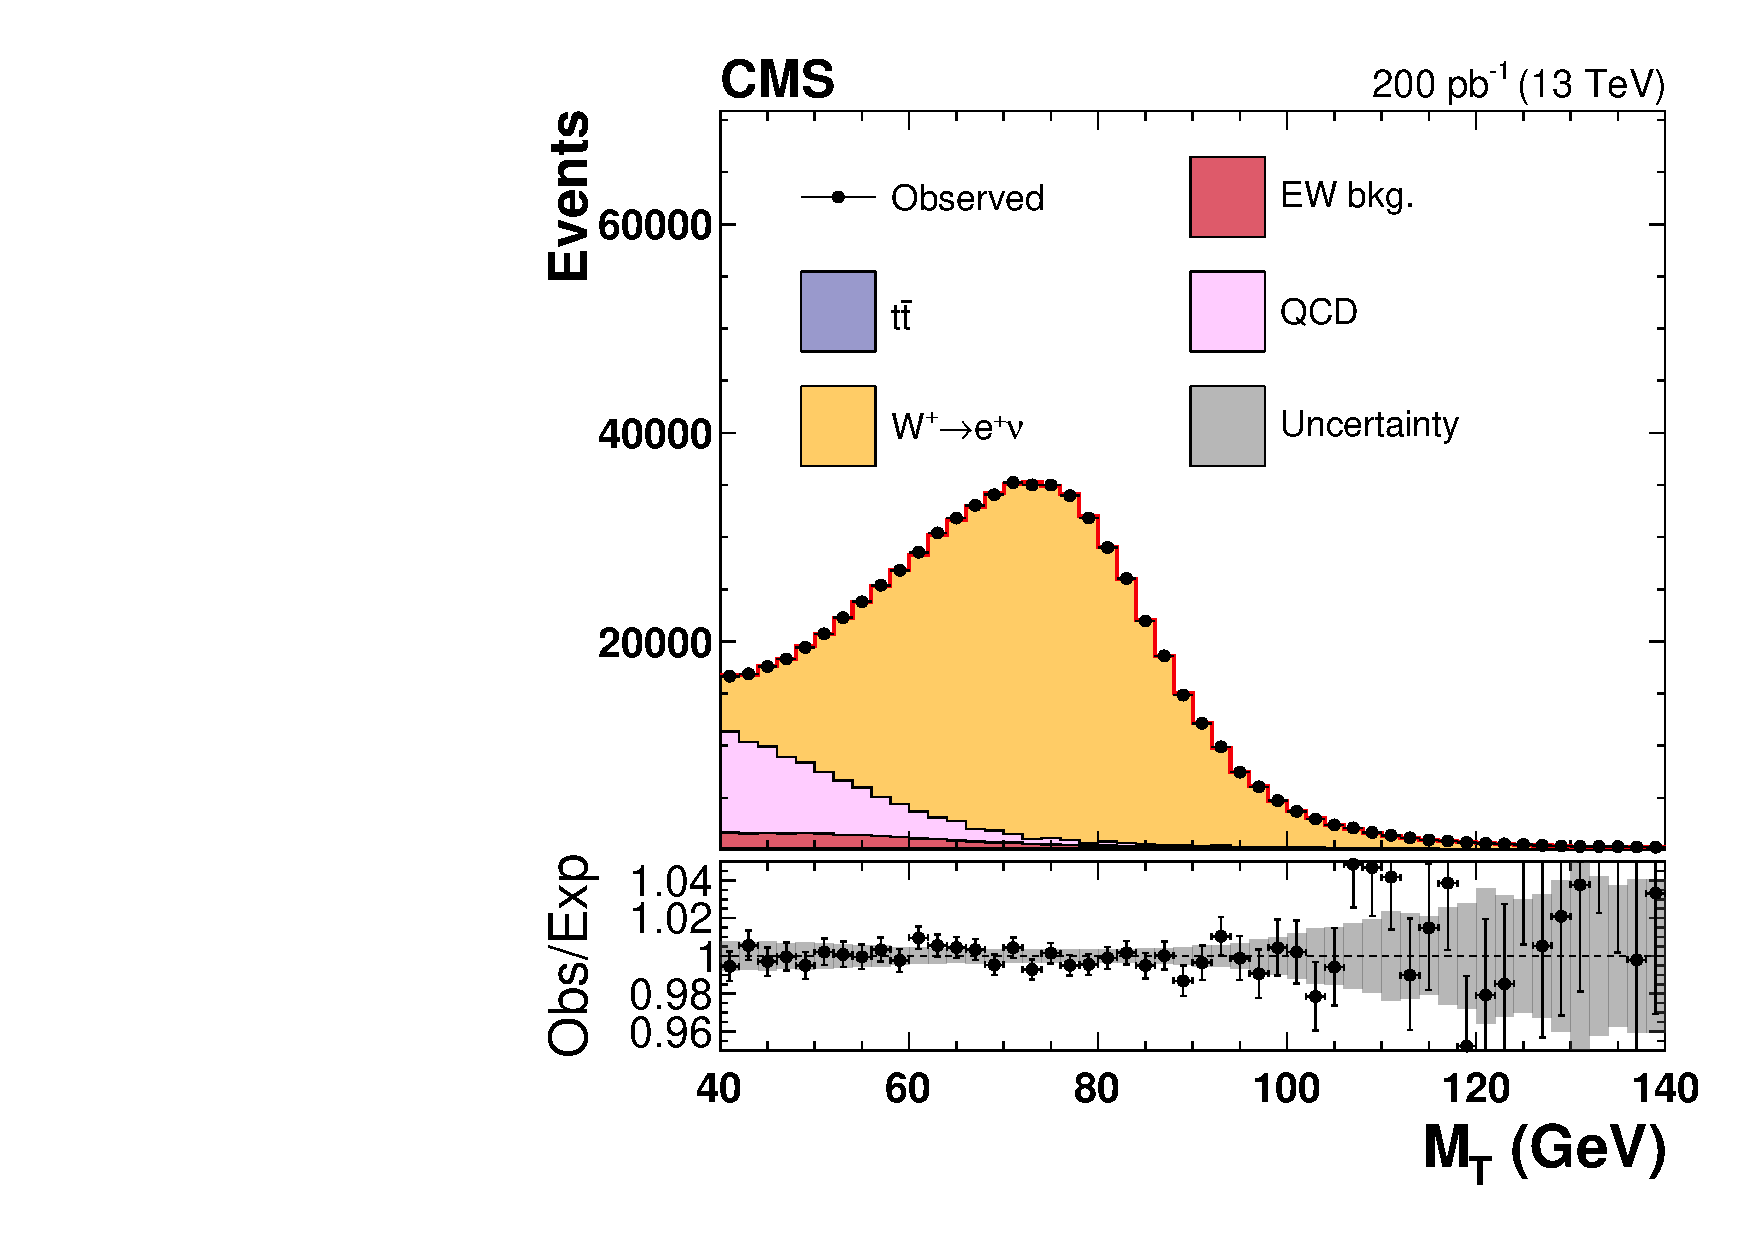
\includegraphics[width=0.49\textwidth]{plots/W/wpefit13.pdf}
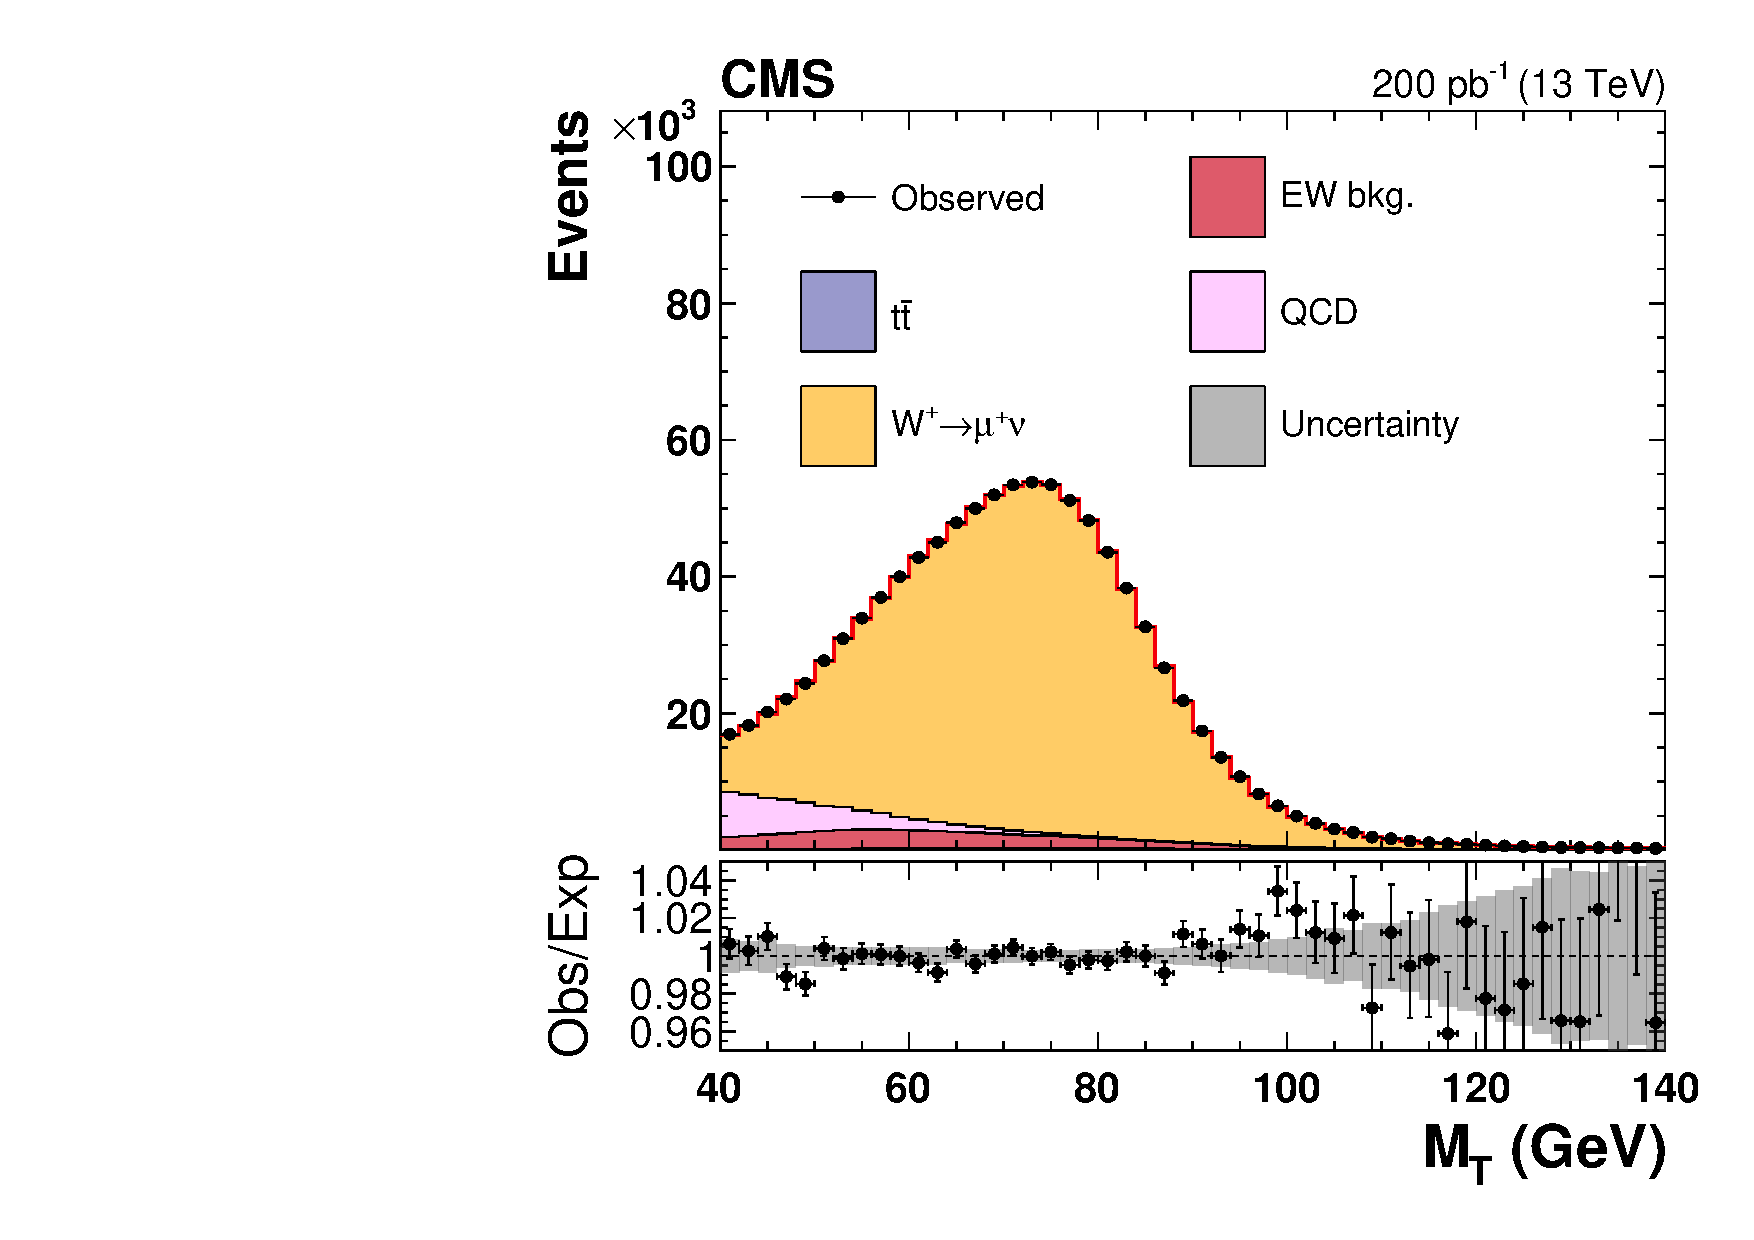
\includegraphics[width=0.49\textwidth]{plots/W/wpmfit13.pdf}
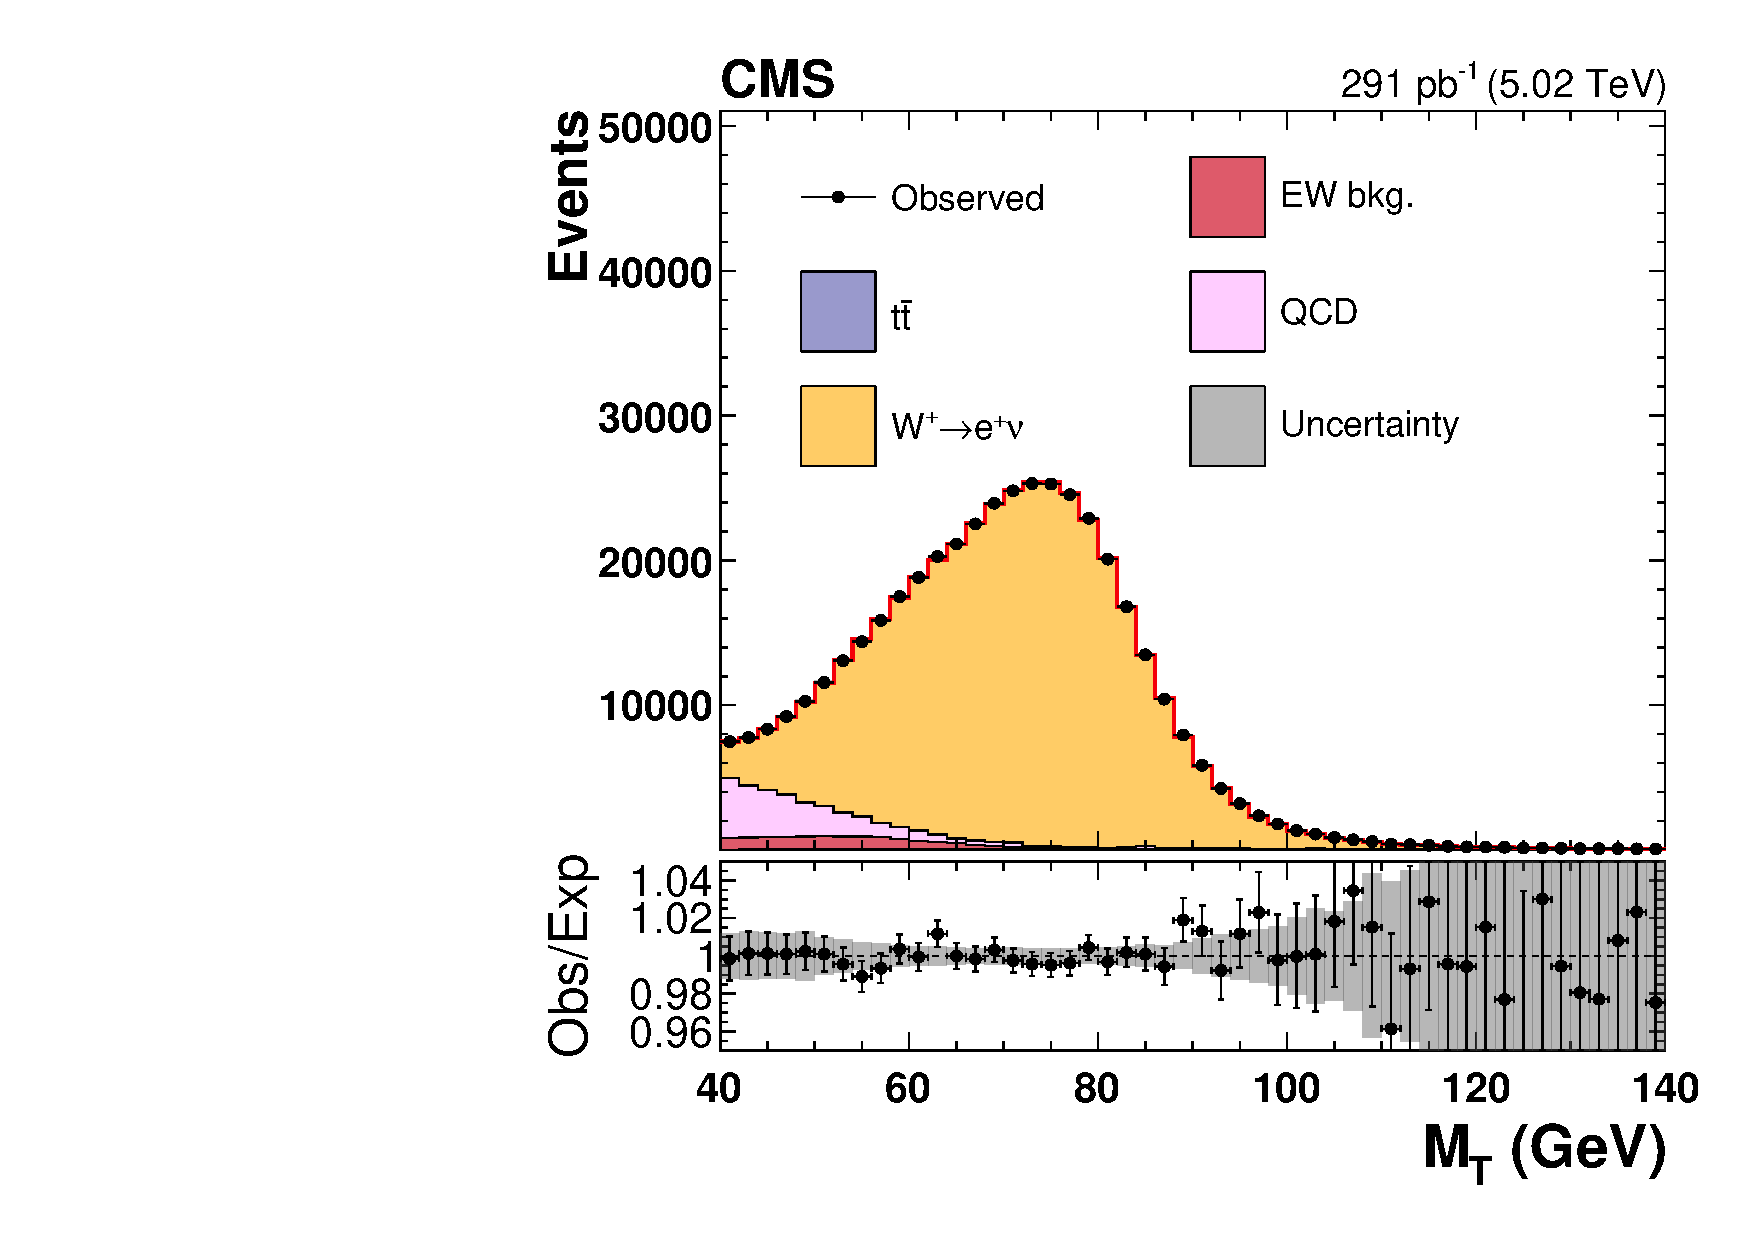
\includegraphics[width=0.49\textwidth]{plots/W/wpefit5.pdf}
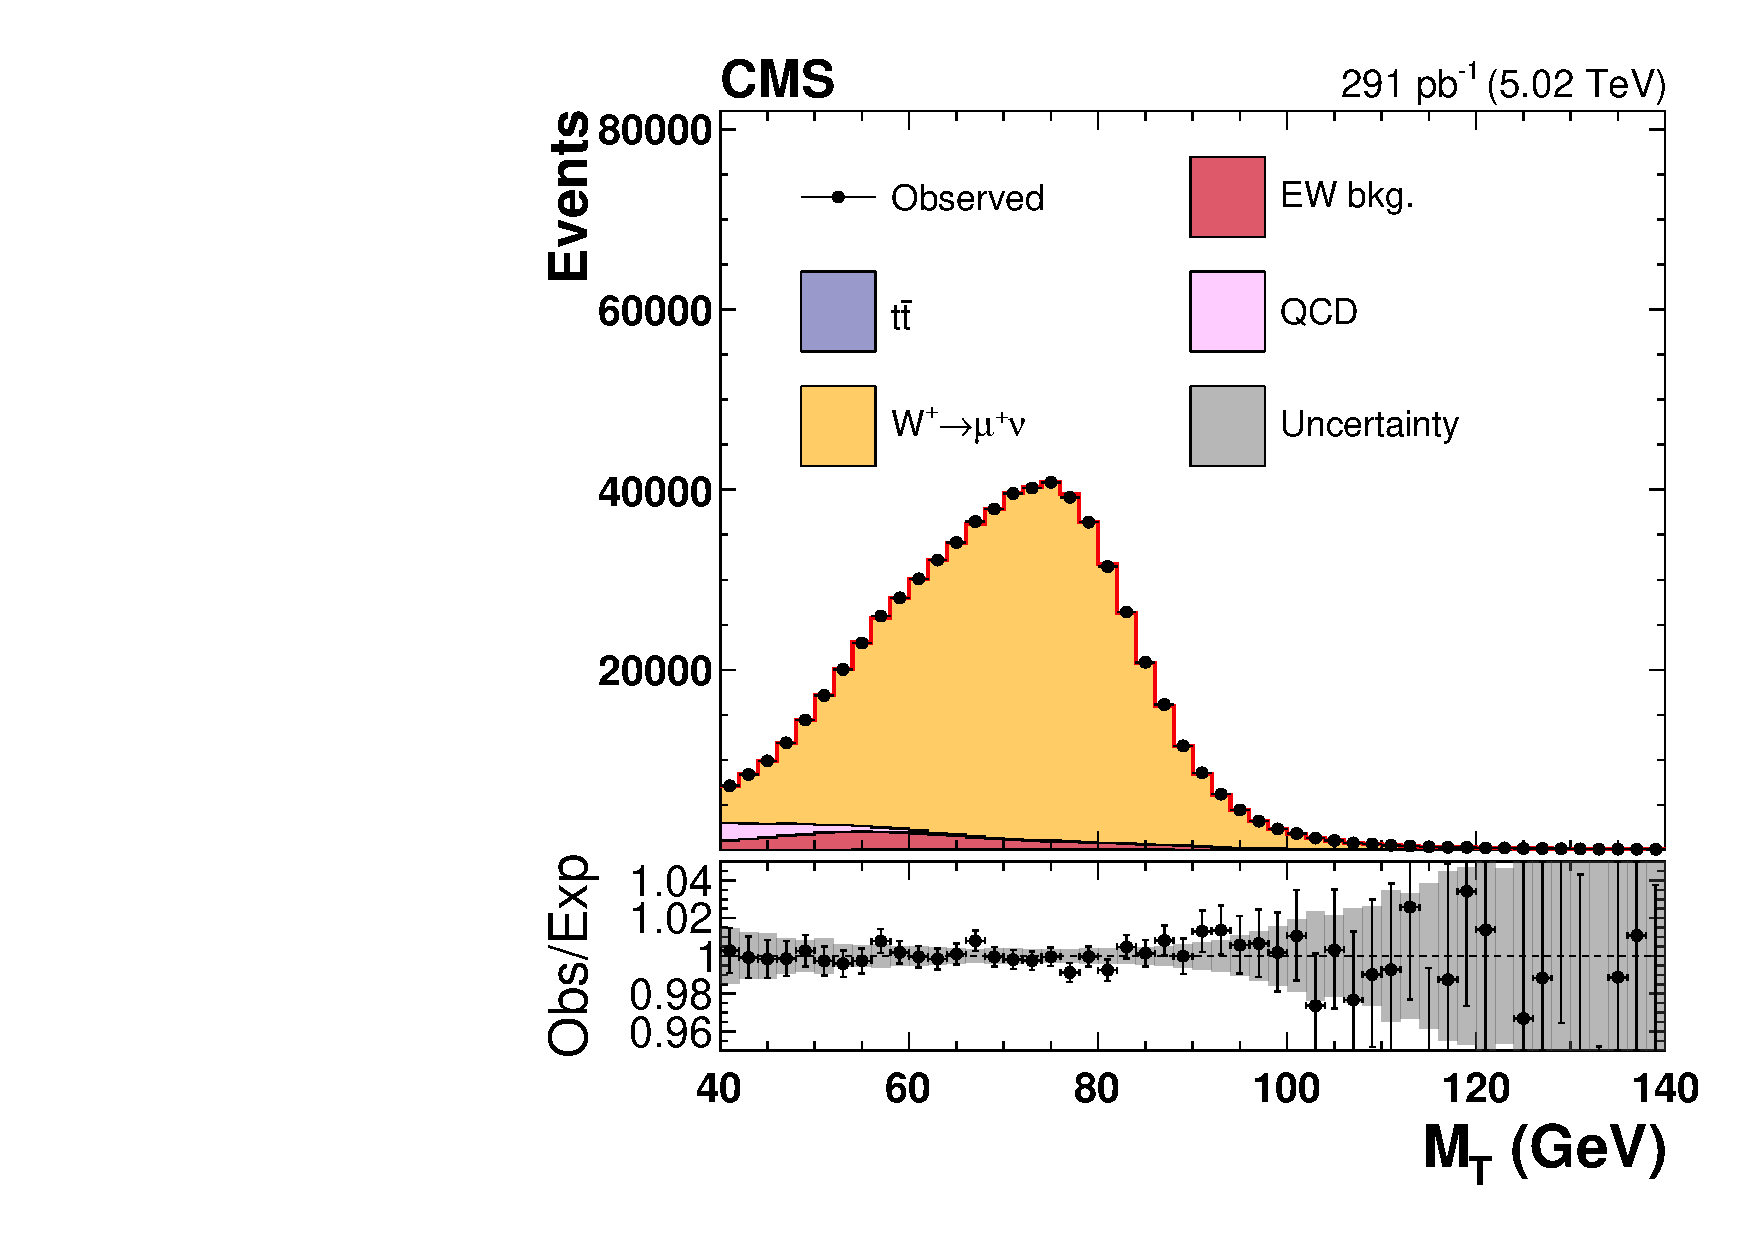
\includegraphics[width=0.49\textwidth]{plots/W/wpmfit5.pdf}
\caption{Distributions of \mt in the $\W^{+}$ signal selection for electron (left) and muon (right) final states for the $pp$ collisions at $\sqrt{s}=13\TeV$ (upper) and $\sqrt{s}=5.02\TeV$ (lower). The histograms for EW backgrounds include the contributions from Drell--Yan, $W \to \tau\nu$, and diboson processes. The predicted yields are shown with their best-fit normalizations from the fit. The bottom panel in each figure shows the ratio of the number of events observed in data to that of the total signal and background predictions.}
\label{fig:signal_wp}
\end{figure*}
\begin{figure*}[htb]
\centering
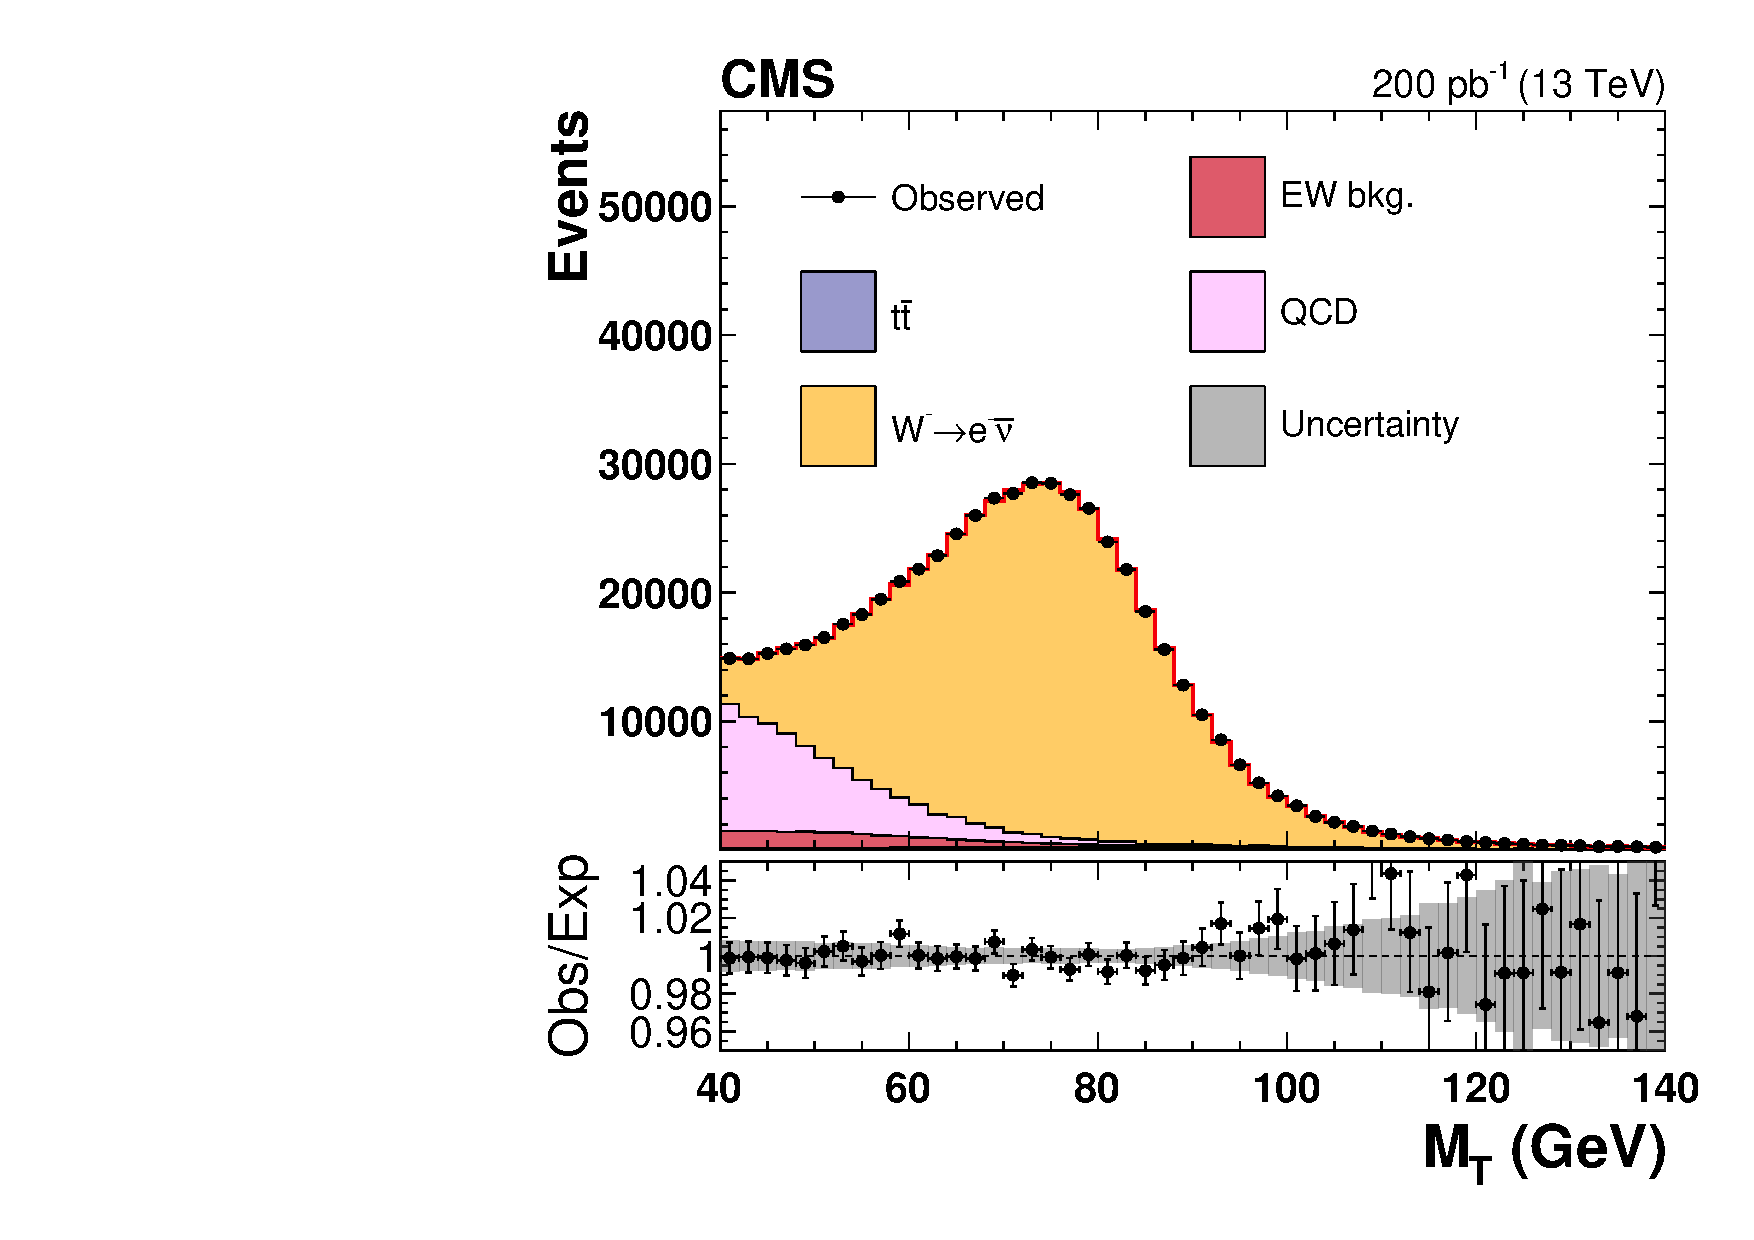
\includegraphics[width=0.49\textwidth]{plots/W/wmefit13.pdf}
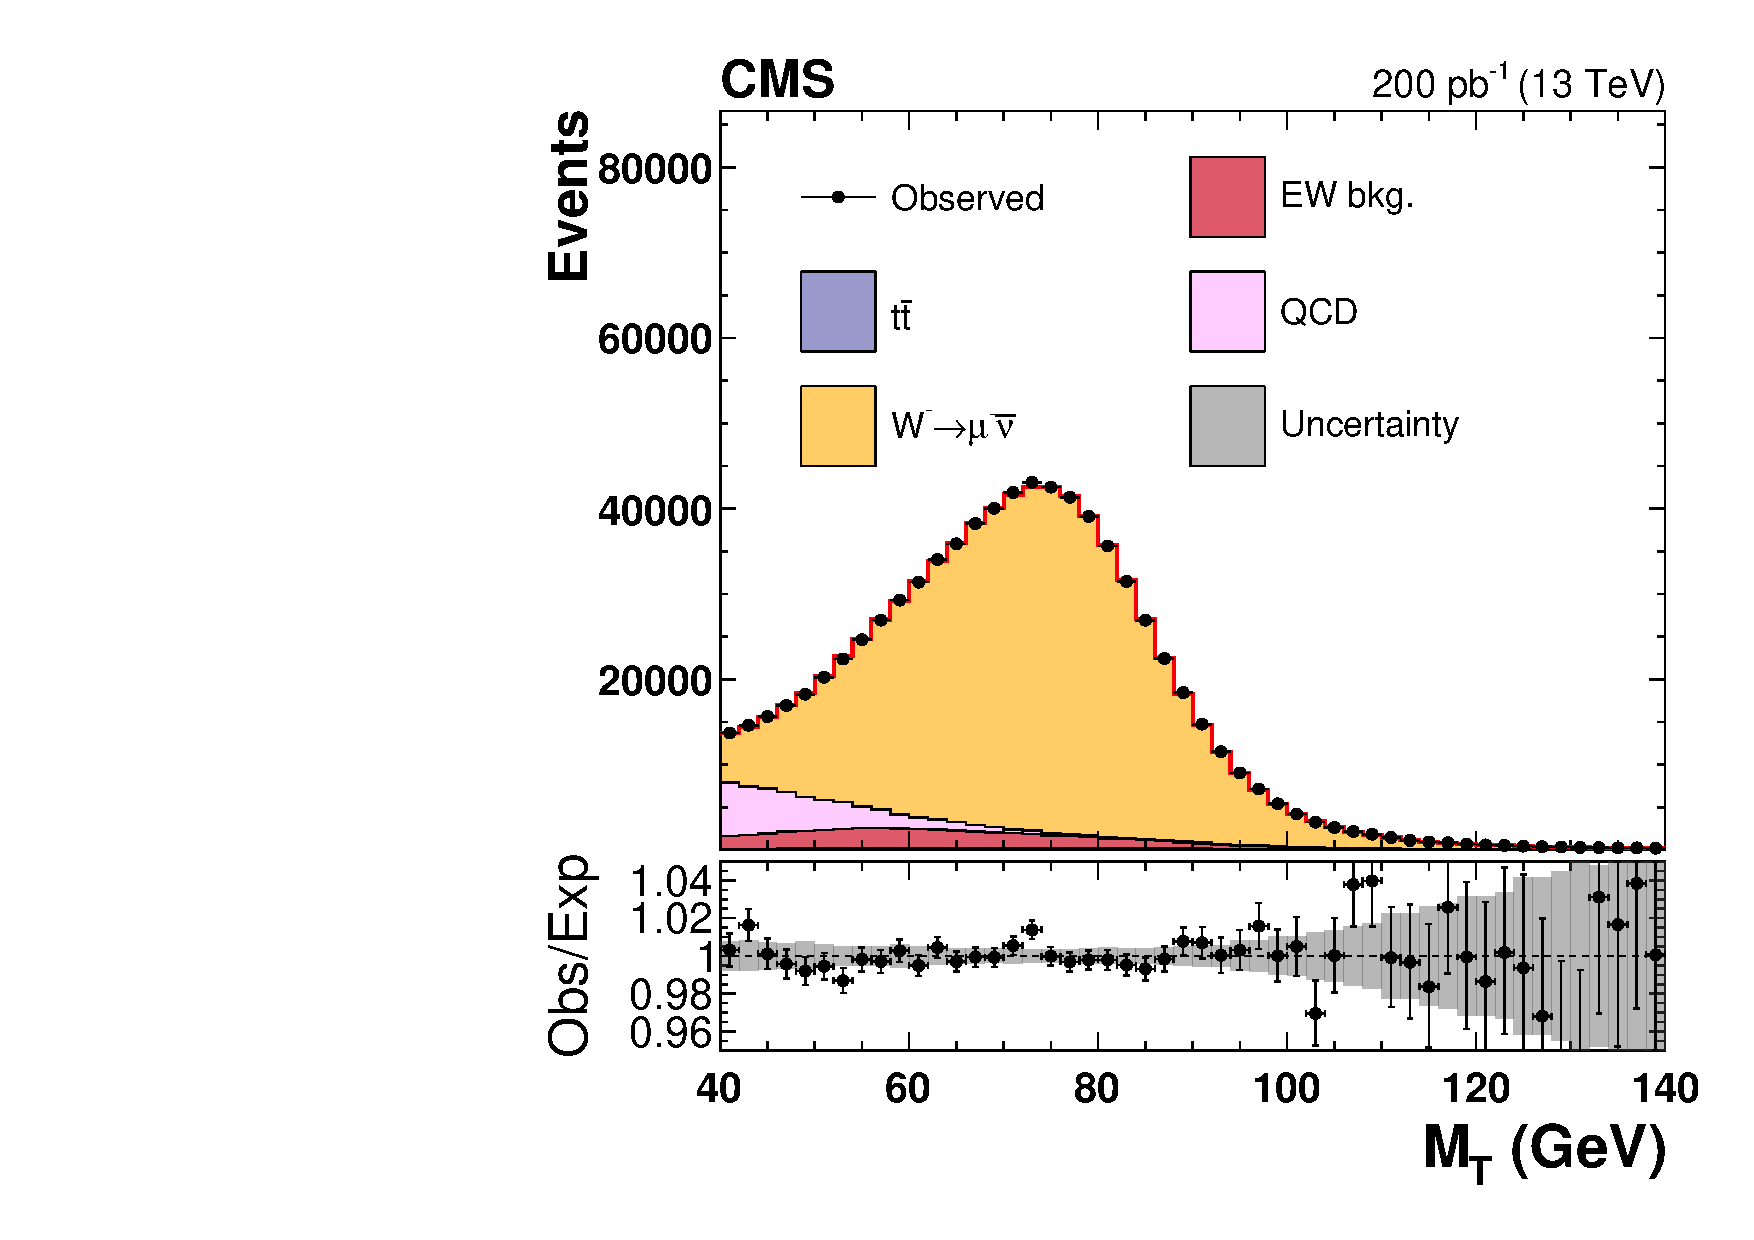
\includegraphics[width=0.49\textwidth]{plots/W/wmmfit13.pdf}
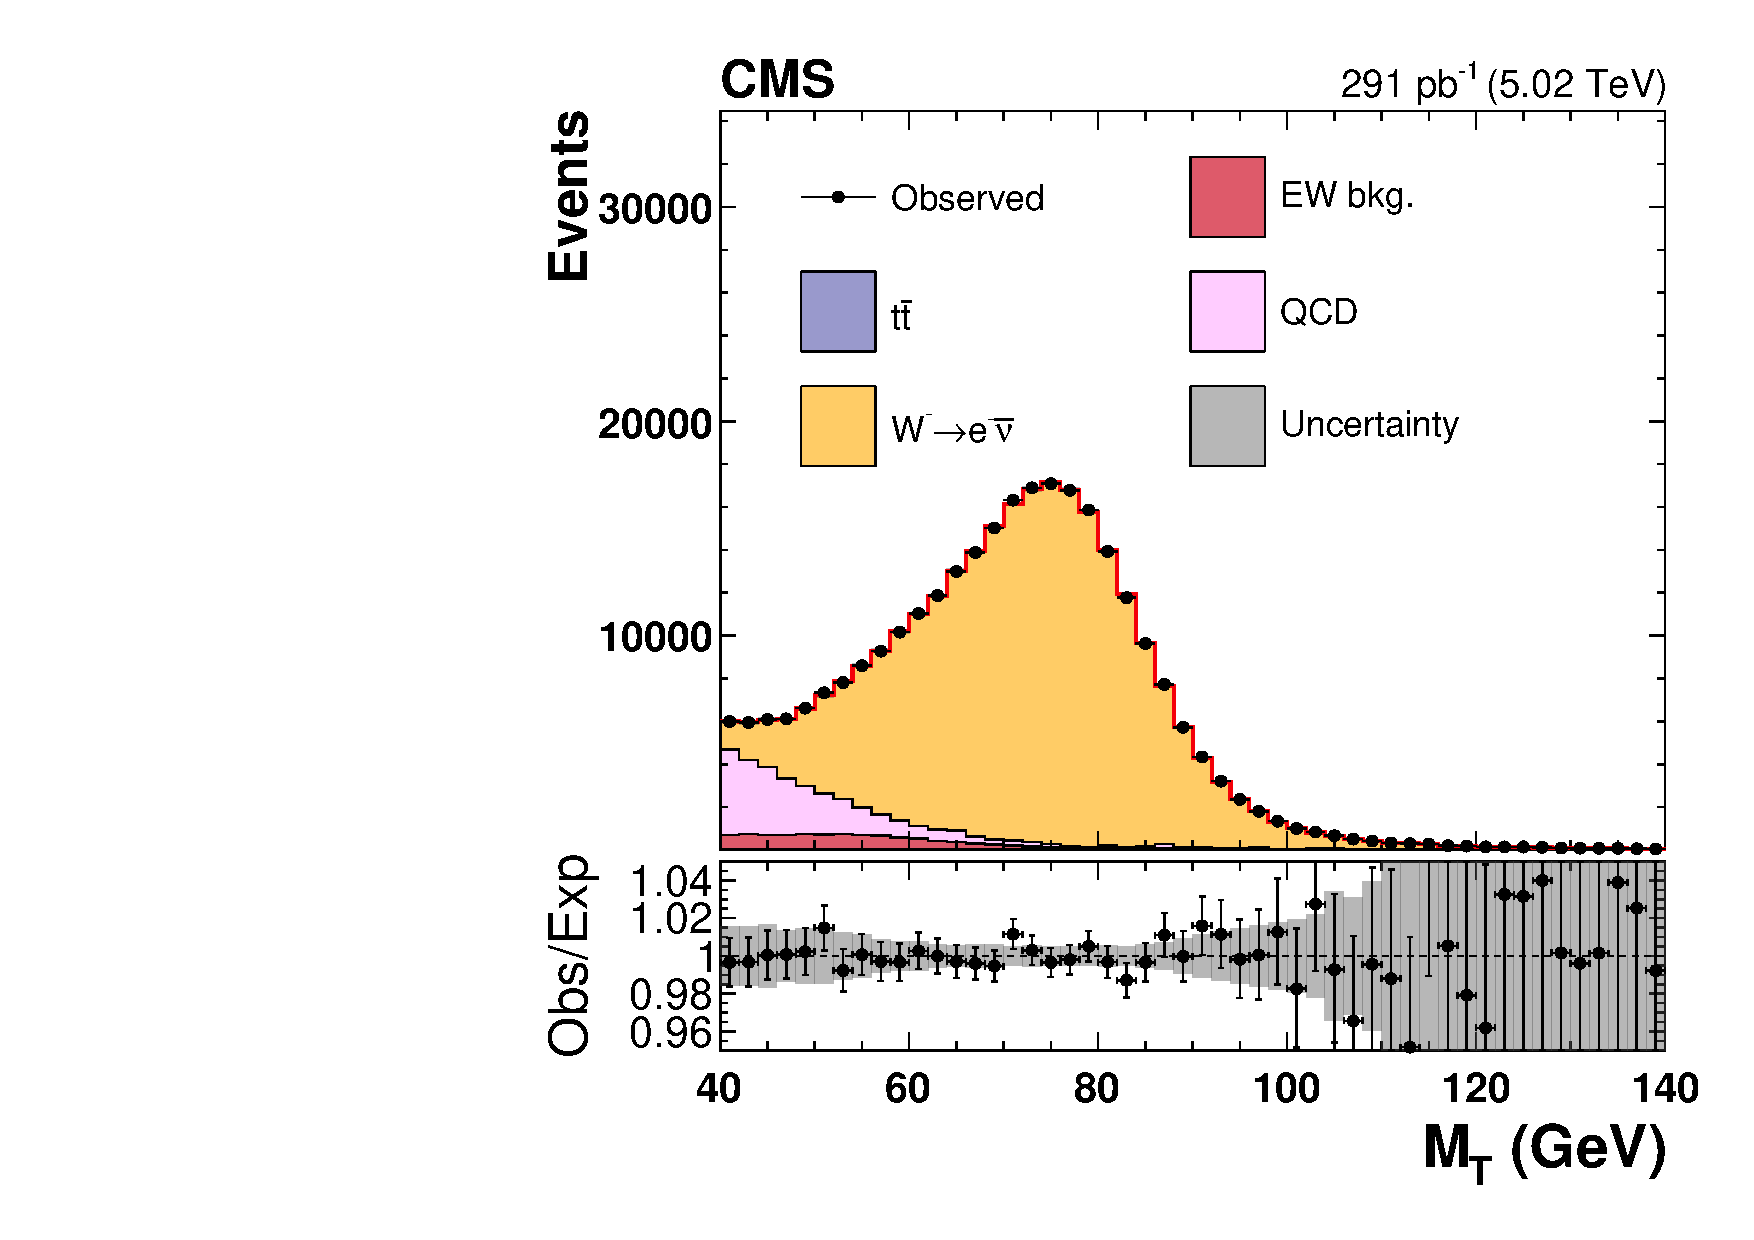
\includegraphics[width=0.49\textwidth]{plots/W/wmefit5.pdf}
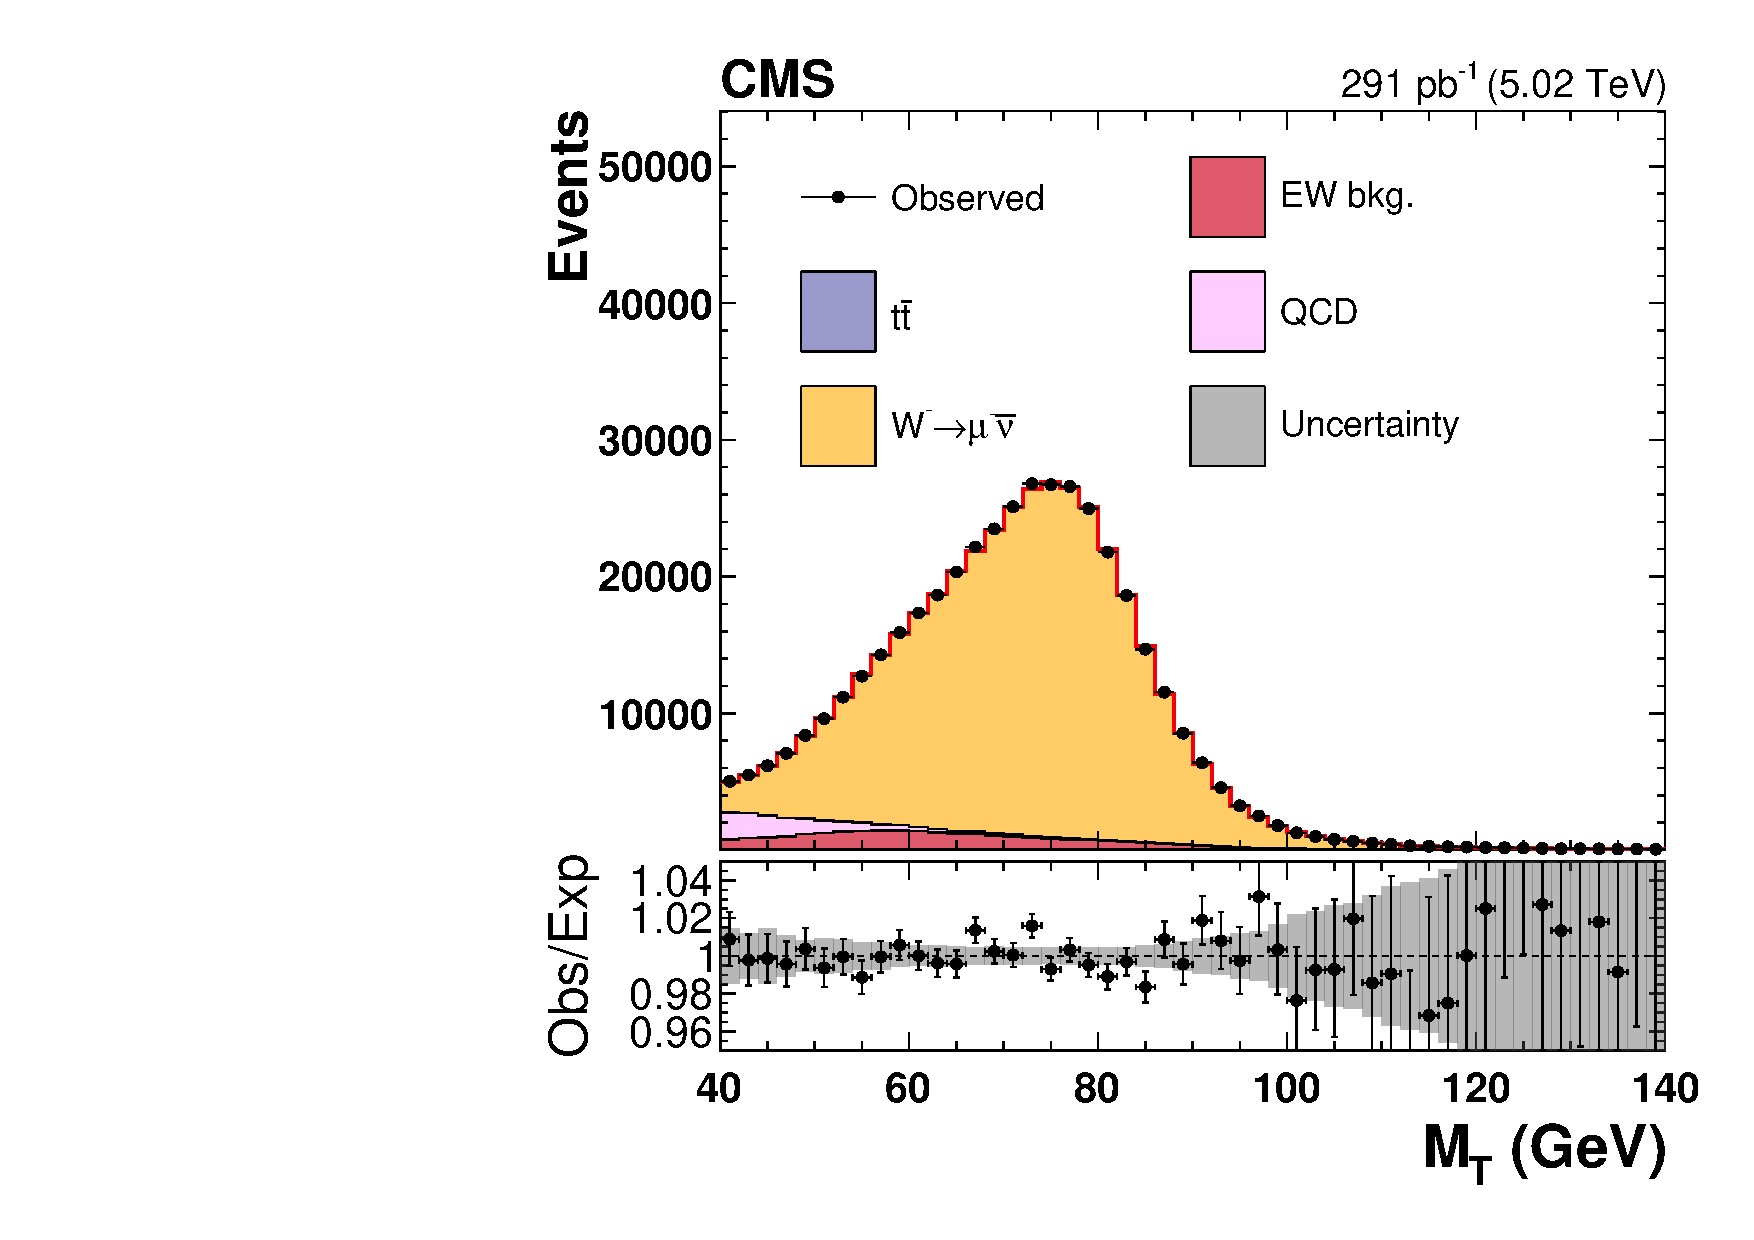
\includegraphics[width=0.49\textwidth]{plots/W/wmmfit5.pdf}
\caption{Distributions of \mt in the $\W^{-}$ signal selection for electron (left) and muon (right) final states for the $pp$ collisions at $\sqrt{s}=13\TeV$ (upper) and $\sqrt{s}=5.02\TeV$ (lower). The histograms for EW backgrounds include the contributions from Drell--Yan, $W \to \tau\nu$, and diboson processes. The predicted yields are shown with their best-fit normalizations from the fit. The bottom panel in each figure shows the ratio of the number of events observed in data to that of the total signal and background predictions.}
\label{fig:signal_wm}
\end{figure*}